% -*- mode:flyspell; mode:latex -*-
\documentclass[12pt]{article}
\addtolength{\oddsidemargin} {-0.885in}
\addtolength{\textwidth}{1.75in}
\addtolength{\evensidemargin}{-0.8in}


\usepackage[latin1]{inputenc}
\usepackage[T1]{fontenc}
\usepackage[english]{babel}
\usepackage{graphicx}
\usepackage{float}
%% \usepackage{siunitx}

%% \usepackage{gensymb}


\usepackage{tikz}
\usepackage{[caption}
\usetikzlibrary{arrows}
\usetikzlibrary{decorations.markings}
\usetikzlibrary{decorations.pathmorphing}
% \usepackage[absolute,overlay]{textpos}
% \usepackage{onimage}

\usepackage{tabularx}
\usepackage{times}
\usepackage{graphics}

% \usepackage{subfigure}
% \usepackage{scalefnt}
%
% \renewcommand\thesubfigure{\arabic{subfigure}}

\usepackage{amsmath}
\usepackage{hyperref}
\usepackage{hhline}
\usepackage{subfig}
\usepackage{color}
\usepackage[all]{hypcap}

\usepackage[normalem]{ulem}  % for striking out
% \usepackage{fancyhdr}
% \pagestyle{fancy}
% \fancyhead[C]{}
% \fancyhead[L] {\it{Mu2e-doc-29670-v1.0} }
%%%%%%%%%%%%%%%%%%%%%%%%%%%%%%%%%%%%%%%%%%%%%%%%%%%%%%%%%%%%%%%%%%%%%%%%%%%%%%
% use natbib - biblatex not available on Mu2e interactive nodes
%%%%%%%%%%%%%%%%%%%%%%%%%%%%%%%%%%%%%%%%%%%%%%%%%%%%%%%%%%%%%%%%%%%%%%%%%%%%%%
\usepackage[square,sort,comma,numbers]{natbib}

% location of the .bib files: env var BIBINPUTS (~/library/bibliography)

% \usepackage[backend=biber, style=numeric-comp, sorting=ynt] {biblatex}
% \addbibresource{clfv.bib}

% \addbibresource{stntuple.bib}
% \addbibresource{mu2e_web.bib}
% \addbibresource{radiative_pion_capture.bib}

\graphicspath{{figures/}}
%%%%%%%%%%%%%%%%%%%%%%%%%%%%%%%%%%%%%%%%%%%%%%%%%%%%%%%%%%%%%%%%%%%%%%%%%%%%%%
% for portability, make sure all commands are included locally,
%%%%%%%%%%%%%%%%%%%%%%%%%%%%%%%%%%%%%%%%%%%%%%%%%%%%%%%%%%%%%%%%%%%%%%%%%%%%%%
\definecolor{ForestGreen}{RGB}{20,109,20}
%\include{commands}
\newcommand {\blue}      {\color{blue}}
\newcommand {\green}     {\color{ForestGreen}}
\newcommand {\red}       {\color{red}}
\newcommand {\purple}    {\color{purple}}
\newcommand {\violet}    {\color{violet}}

\newcommand {\kmax}      {\mbox{$k_{\rm max}$}}
\newcommand {\piplusenu} {\mbox{$\pi^+ \to e^+ \nu$}}

\newcommand {\mumemconv}[1][A] {\mbox{$\mu^- \textrm{#1} \rightarrow e^- \textrm{#1}$}}
% Define a relay to have 2 default arguments instead of limit of 1
\newcommand {\mumepconv}[1][A] {%
  \def\ArgI{{#1}}%store the first argument
  \mumepconvRelay
}
\newcommand \mumepconvRelay[1][A]  {\mbox{$\mu^- \textrm{\ArgI} \rightarrow e^+ \textrm{#1}$}}
\newcommand {\MuToEm}     {\mbox{$\mu^- \ra e^-$}}
\newcommand {\MuToEp}     {\mbox{$\mu^- \ra e^+$}}
\newcommand {\MuPToEp}    {\mbox{$\mu^+ \ra e^+$}}
\newcommand {\ra}        {\rightarrow}
\newcommand {\Rmue}       {\mbox{$R_{\mu e}$}}
\newcommand {\tandip}    {\mbox{$\tan \lambda$}}

\newcommand {\Pb}[1]     {\mbox{$\rm ^{#1}Pb$}}                 % isotopes of lead
\newcommand {\Au}[1]     {\mbox{$\rm ^{#1}Au$}}                 % isotopes of gold
\newcommand {\Ir}[1]     {\mbox{$\rm ^{#1}Ir$}}                 % isotopes of iridium
%%%%%%%%%%%%%%%%%%%%%%%%%%%%%%%%%%%%%%%%%%%%%%%%%%%%%%%%%%%%%%%%%%%%%%%%%%%%%%
% editing commands
%%%%%%%%%%%%%%%%%%%%%%%%%%%%%%%%%%%%%%%%%%%%%%%%%%%%%%%%%%%%%%%%%%%%%%%%%%%%%%
\newcommand {\del}[1]    {{\blue   \sout{#1}}}
\newcommand {\dlt}[1]    {{\violet \sout{#1}}} %alternate delete color
\newcommand {\add}[1]    {{\red #1}}
\newcommand {\alt}[1]    {{\green #1}} %alternate comment color
% %%%%%%%%%%%%%%%%%%%%%%%%%%%%%%%%%%%%%%%%%%%%%%%%%%%%%%%%%%%%%%%%%%%%%%%%%%%%%%
% for editors
% %%%%%%%%%%%%%%%%%%%%%%%%%%%%%%%%%%%%%%%%%%%%%%%%%%%%%%%%%%%%%%%%%%%%%%%%%%%%%%
\newcommand {\pasha}[1]    {{\green  #1}}
\newcommand {\kate}[1]     {{\blue   #1}}
%%%%%%%%%%%%%%%%%%%%%%%%%%%%%%%%%%%%%%%%%%%%%%%%%%%%%%%%%%%%%%%%%%%%%%%%%%%%%%
\begin{document}

\begin{titlepage}
  \begin{flushright}
    \bf {MU2E/PHYSICS/50071} \\
    version 1.01
    \today
 \end{flushright}

  \vspace{1cm}

  \begin{center}
    {\Large \bf On a possibility of the Mu2e momentum scale calibration at full field
      \vspace{0.3in}
      1. Initial analysis
    }

    \vspace{1cm}
    K.Ciampa(BU), P.Murat(FNAL)

    % \footnote{\texttt{Fermilab; e-mail: murat@fnal.gov}}
    \vspace{0.3cm}

    \vspace{0.8cm}
  \end{center}

  \begin{abstract}
    \vspace{0.2in}
    Radiative pion capture (RPC) on hydrogen  provides a unique opportunity to calibrate
    the Mu2e momentum scale at full field.

    Kinematic edge of the momentum distribution of 129.4 MeV RPC photons
    reconstructed in $\gamma \to e^+e^-$ channel could be used as a calibration line.

    We investigate whether the rate of events of interest is sufficient for the calibration.

    Color legend:
    
    \begin{itemize}
    \item
      \kate{color for Kate}
    \item 
      \pasha{color for Pasha}
    \item
      {\red color for TODO items}
    \end{itemize}

      \end{abstract}

\end{titlepage}
% \frontmatter
% \chapter*{Abstract}
%
% \addcontentsline{toc}{chapter}{Abstract}
%
% \mainmatter
%
{\tableofcontents}

%%%%%%%%%%%%%%%%%%%%%%%%%%%%%%%%%%%%%%%%%%%%%%%%%%%%%%%%%%%%%%%%%%%%%%%%%%%%%%%
%\chapter{Calibration}
%%%%%%%%%%%%%%%%%%%%%%%%%%%%%%%%%%%%%%%%%%%%%%%%%%%%%%%%%%%%%%%%%%%%%%%%%%%%%%%
% \input{input_data}

%%%%%%%%%%%%%%%%%%%%%%%%%%%%%%%%%%%%%%%%%%%%%%%%%%%%%%%%%%%%%%%%%%%%%%%%%%%%%%%

\newpage
\section {Revision History and TODO items}

\begin{itemize}
\item
  v1.01: inital version
\end{itemize}

TODO items:

\begin{itemize}
\item
  placeholder
\end{itemize}

%%%%%%%%%%%%%%%%%%%%%%%%%%%%%%%%%%%%%%%%%%%%%%%%%%%%%%%%%%%%%%%%%%%%%%%%%%%%%%
\newpage
\section {Introduction}

%%%%%%%%%%%%%%%%%%%%%%%%%%%%%%%%%%%%%%%%%%%%%%%%%%%%%%%%%%%%%%%%%%%%%%%%%%%%%%
\section{RPC on hydrogen}

Has been measured in \cite{RPC_1972_Bistirlich_PhysRevC.5.1867}.

{\red
  \begin{itemize}
  \item 
    need an estimate of the fraction of stopped pions captured by hydrogen
  \item
    after that is determined, use spectrum on CH2 to generate photons
  \end{itemize}
}
%%% Local Variables:
%%% mode: latex
%%% TeX-master: t
%%% End:

%%%%%%%%%%%%%%%%%%%%%%%%%%%%%%%%%%%%%%%%%%%%%%%%%%%%%%%%%%%%%%%%%%%%%%%%%%%%%%
\section{$\pi^- p \to n \gamma$ photons as a calibration line}

Photons from RPC on hydrogen could be used to calibrate the Mu2e momentum scale and, simultaneously, measure the momentum resolution.
Consider a RPC  photon converting in the detector material 
and producing an $e^+e^-$ pair. In case of a symmetric conversion, the momenta of both particles
are $\sim$ 65 MeV/c. If the conversion radius is large enough, both an electron
and a positron from $\gamma \to e^+ e^-$ may produce enough hits in the tracker
so their tracks could be reconstructed and used to reconstruct the momentum of the
converted photon.

Acceptance is maximized for photons emitted at $90^o$ with respect to the DS axis. 

The Mu2e detector has a component, the pion degrader, which with small modifications
could be used for this calibration measurement. The degrader was initially introduced
in order to suppress the background to \piplusenu\ from muon decays
in flight \cite{MU2E_2527_PIPLUSENU},
It is a movable disk made of non-magnetic material, which gets inserted into
the beam during the calibration runs and moved out of the beam during
the regular data taking.

Making the degrader disk out of polyethylene and surrounding it, at a larger radius, 
with a thin converter foil could allow to convert photons emitted at angles close to $90^o$
with respect to the DS axis. A schematic view of the modified degrader geometry is presented in Figure~\ref{figure:degrader_geometry_v3}.

The converter foil could be supported by a light carbon foam disk mounted on the degrader.

\begin{figure}[H]
  \begin{tikzpicture}
    \node[anchor=south west,inner sep=0] at (0,-10.) {
      % \node[shift={(0 cm,0.cm)},inner sep=0,rotate={90}] at (0,0) {}
      \makebox[\textwidth][c] {
        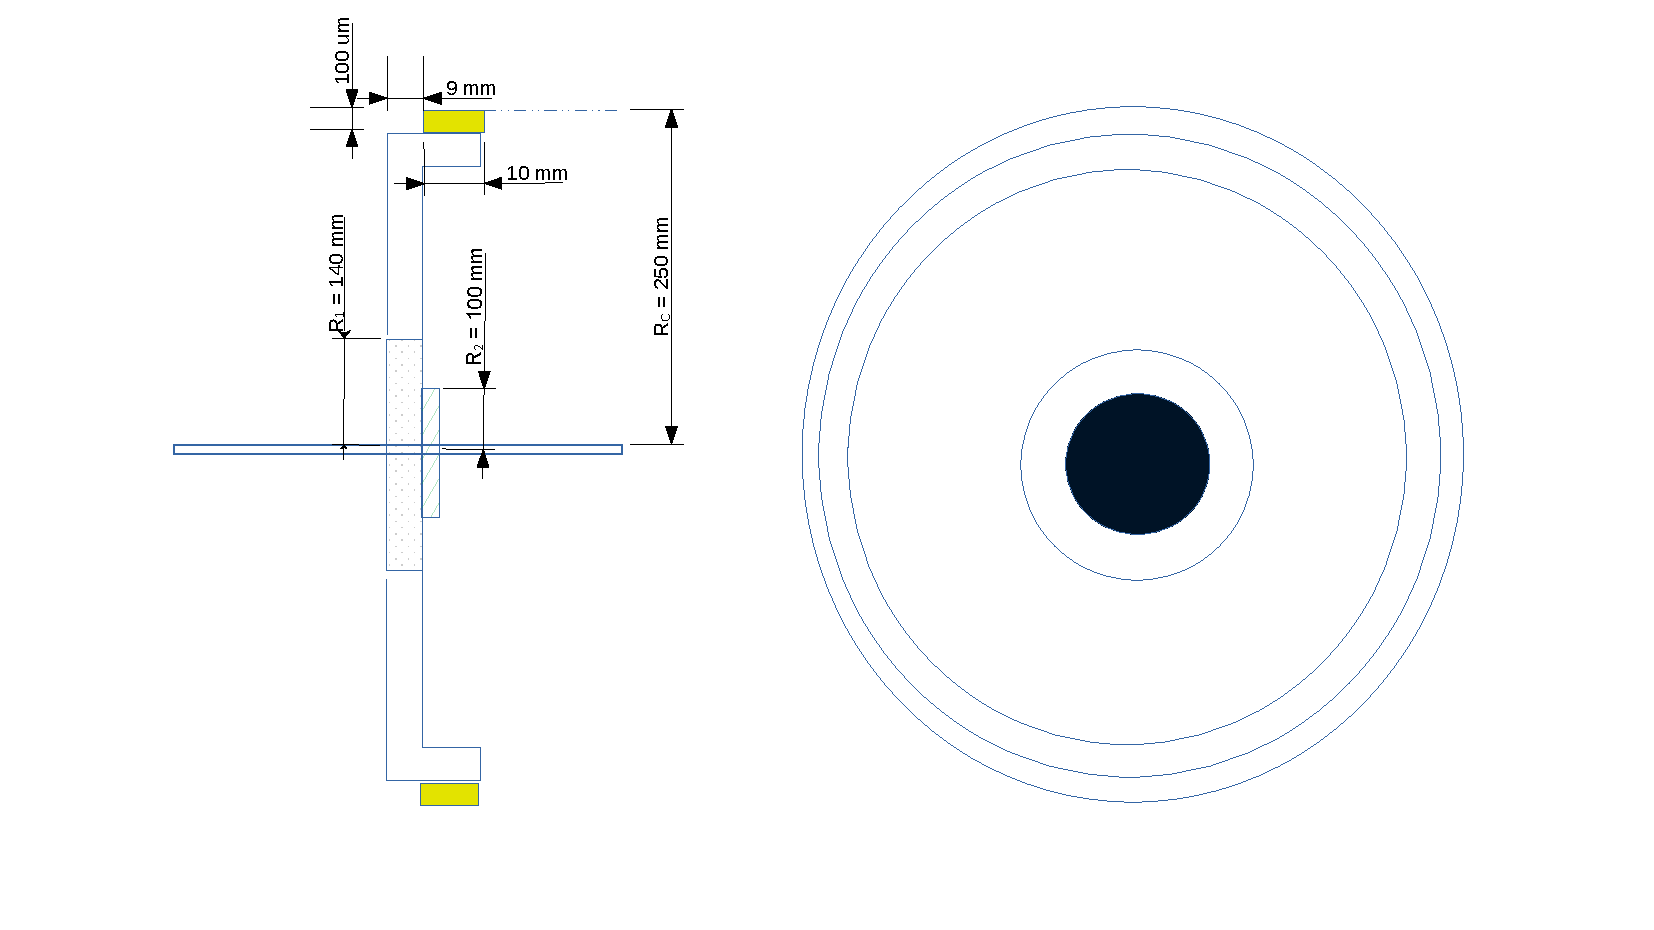
\includegraphics[width=0.95\textwidth]{pdf/degrader_geometry_002}
      }
    };
    % \node [text width=8cm, scale=1.0] at (14.5,0.5) {$\mu_B$, expected background mean};
    % \node [text width=8cm, scale=1.0, rotate={90}] at (1.5,7.5) { $S_{D}$, ``discovery'' signal strength  };
  \end{tikzpicture}
  \caption{
    \label{figure:degrader_geometry_v3}
    Schematic view of the simulated degrader geometry, not up to scale
  }
\end{figure}

%%%%%%%%%%%%%%%%%%%%%%%%%%%%%%%%%%%%%%%%%%%%%%%%%%%%%%%%%%%%%%%%%%%%%%%%%%%%%%
\subsection{Simulation} 
A configuration of the Mu2e detector with the pion degrader, as shown in  Figure~\ref{figure:degrader_geometry_v3}, inserted in the beam has been simulated.

\begin{itemize}
\item 
  From \piplusenu\ studies: the pion degrader disk thickness of 4 mm Ti is close to optimal.
\item
  4mm of Ti translates into the total amount of material of $\sim 1.8 g/cm^2$,
  about twice the material of the stopping target.
\item
  9mm CH2 + 1.0mm Pb: : 2.0 $g/cm^2$   .. $\pi*15^2*(0.9*0.95 + 0.08*11.34): \simeq 2 g/cm^2$
\item
   9mm CH2 + 0.8mm Pb: : $1.76 g/cm^2$
 \item
   CH2 disk R=14 cm, weight        : $0.90*0.95*\pi*14^2 ~= 526$ gr \\
   Pb  foil R=10cm thickness 0.8mm : $0.08*11.34*\pi*10^2 = 285$ gr \\
   total                           : 811 gr
 \item 
   The gold converter ring has the outer radius $R_{out}$ = 250mm,
   and the value of $R_{in}$ is defined by the converter thickness.
   The converter is slightly offset downstream with respect to the $CH_2$ disk,
   so $e*+$ and $e^-$ produced in the converter do not cross it multiple times.

\end{itemize}

For small, of the order of few cm, widths of the converter ring,
the acceptance is proportional to the width.
So making teh width, for example, 3cm instead of 1 cm wide would increase
the acceptance by a factor close to x3. However, the space between the OPA
and the TS available
for the degrader installation is limited, about 5 cm along the Z axis, 
and that limits the maximal width of the converter ring. Also, a large radius
of the converter ring, R = 25-30 cm, could start limiting the movement of the
degrader arm.

A potentially more attractive alternative could be to have the converter placed
on a thin carbon foam ring and supported inside the OPA. In this case,
the width of the foil could be increased without introducing the space conflicts.
Having the converter supported by the OPA would also simplify increasing
the converter radius should that become necessary.
%
This option is discussed in Section~\ref{section:geometry_v4}


%%%%%%%%%%%%%%%%%%%%%%%%%%%%%%%%%%%%%%%%%%%%%%%%%%%%%%%%%%%%%%%%%%%%%%%%%%%%%%
\subsection{Stopped negative pions}

Simulation of the negative pion beam follows the standard 2-stage model.
Stage 2 produces three separate datasets of pions stops in the CH2, Pb, and the ST.
The scheme allow to resimulate the pion stop datasets w/o repeating more time consuming
first stage of the simulation.
To improve the simulation efficiency pion decays are disabled. The calculated by Geant4
pion survival probabilities are used as event weights in the normalization procedure.

Distributions of momentum and time for pions stopped in it CH2, Pb foil, and the
stopping target are shown in Figure \ref{figure:stopped_pim_mom_time}.

\begin{figure}[H]
  \begin{tikzpicture}
    \node[anchor=south west,inner sep=0] at (0,0.) {
      % \node[shift={(0 cm,0.cm)},inner sep=0,rotate={90}] at (0,0) {}
      % \makebox[\textwidth][c] {
        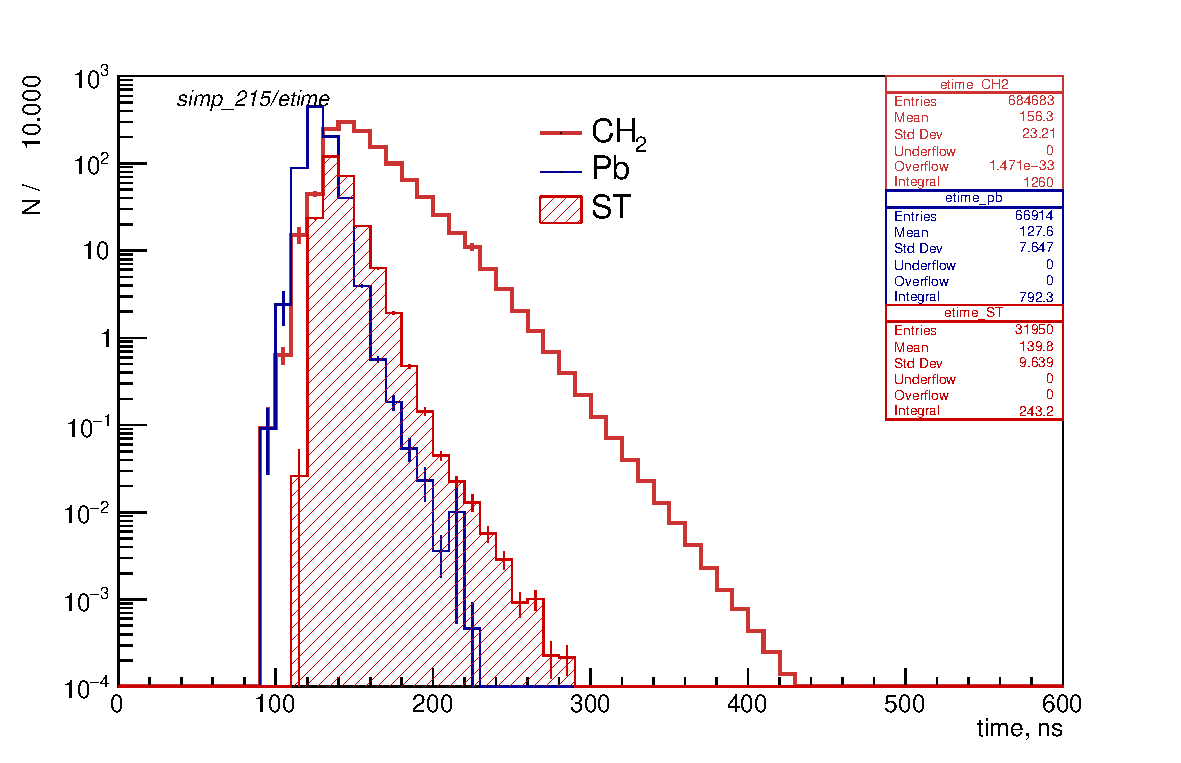
\includegraphics[width=0.5\textwidth]{pdf/figure_00021}
      % }
    };
    \node[anchor=south west,inner sep=0] at (10,0.) {
      % \node[shift={(0 cm,0.cm)},inner sep=0,rotate={90}] at (0,0) {}
      % \makebox[\textwidth][c] {
        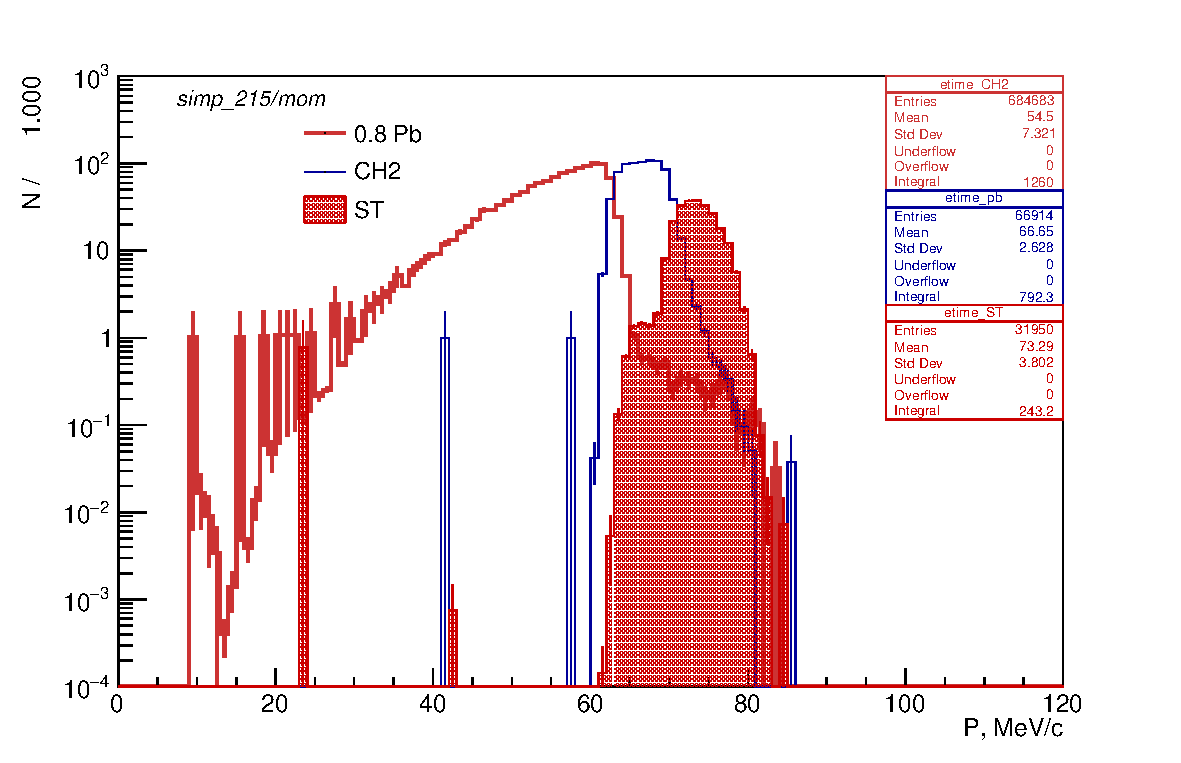
\includegraphics[width=0.5\textwidth]{pdf/figure_00022}
      % }
    };
    % \node [text width=8cm, scale=1.0] at (14.5,0.5) {$\mu_B$, expected background mean};
    % \node [text width=8cm, scale=1.0, rotate={90}] at (1.5,7.5) { $S_{D}$, ``discovery'' signal strength  };
  \end{tikzpicture}
  \caption{
    \label{figure:stopped_pim_mom_time}
    Stopped pions: distributions of momentum and time
  }
\end{figure}

It is worth noting that pions stopped in the $CH_2$ are the slowest ones.
Therefore, selecting events with the pion stop time above certain threshold, i.e. $\sim 200$ ns, 
significantly suppresses contributions of the stopping target and the Pb foil to any measurement.
T0 = 200 ns is also approximately the time where the instantaneous beam flash
hit rate gets reduced down to the level allowing the measurements. For the DAQ operations,
that means that the digitization start time should be lowered to $\sim 250$ ns,
which, at a reduced proton beam intensity, looks quite realistic.

Another interesting correlation is the correlation between the pion momentum on exit from the TS momentum
and the vertical coordinate of the pion stop point. Figure ~\ref{figure:y_vs_p_deg} shows this correlation
for pions stopped in the $CH_2$ and Pb parts of the degrader. The Y distribution of the pion stops
in the Pb foil is offset down by several centimeters. The lower cut-off at R=100 mm is determined by the
by the simulated radius of the Pb foil, R=100mm

\begin{figure}[H]
  \begin{tikzpicture}
    \node[anchor=south west,inner sep=0] at (0,0.) {
      % \node[shift={(0 cm,0.cm)},inner sep=0,rotate={90}] at (0,0) {}
      %\makebox[\textwidth][c] {
        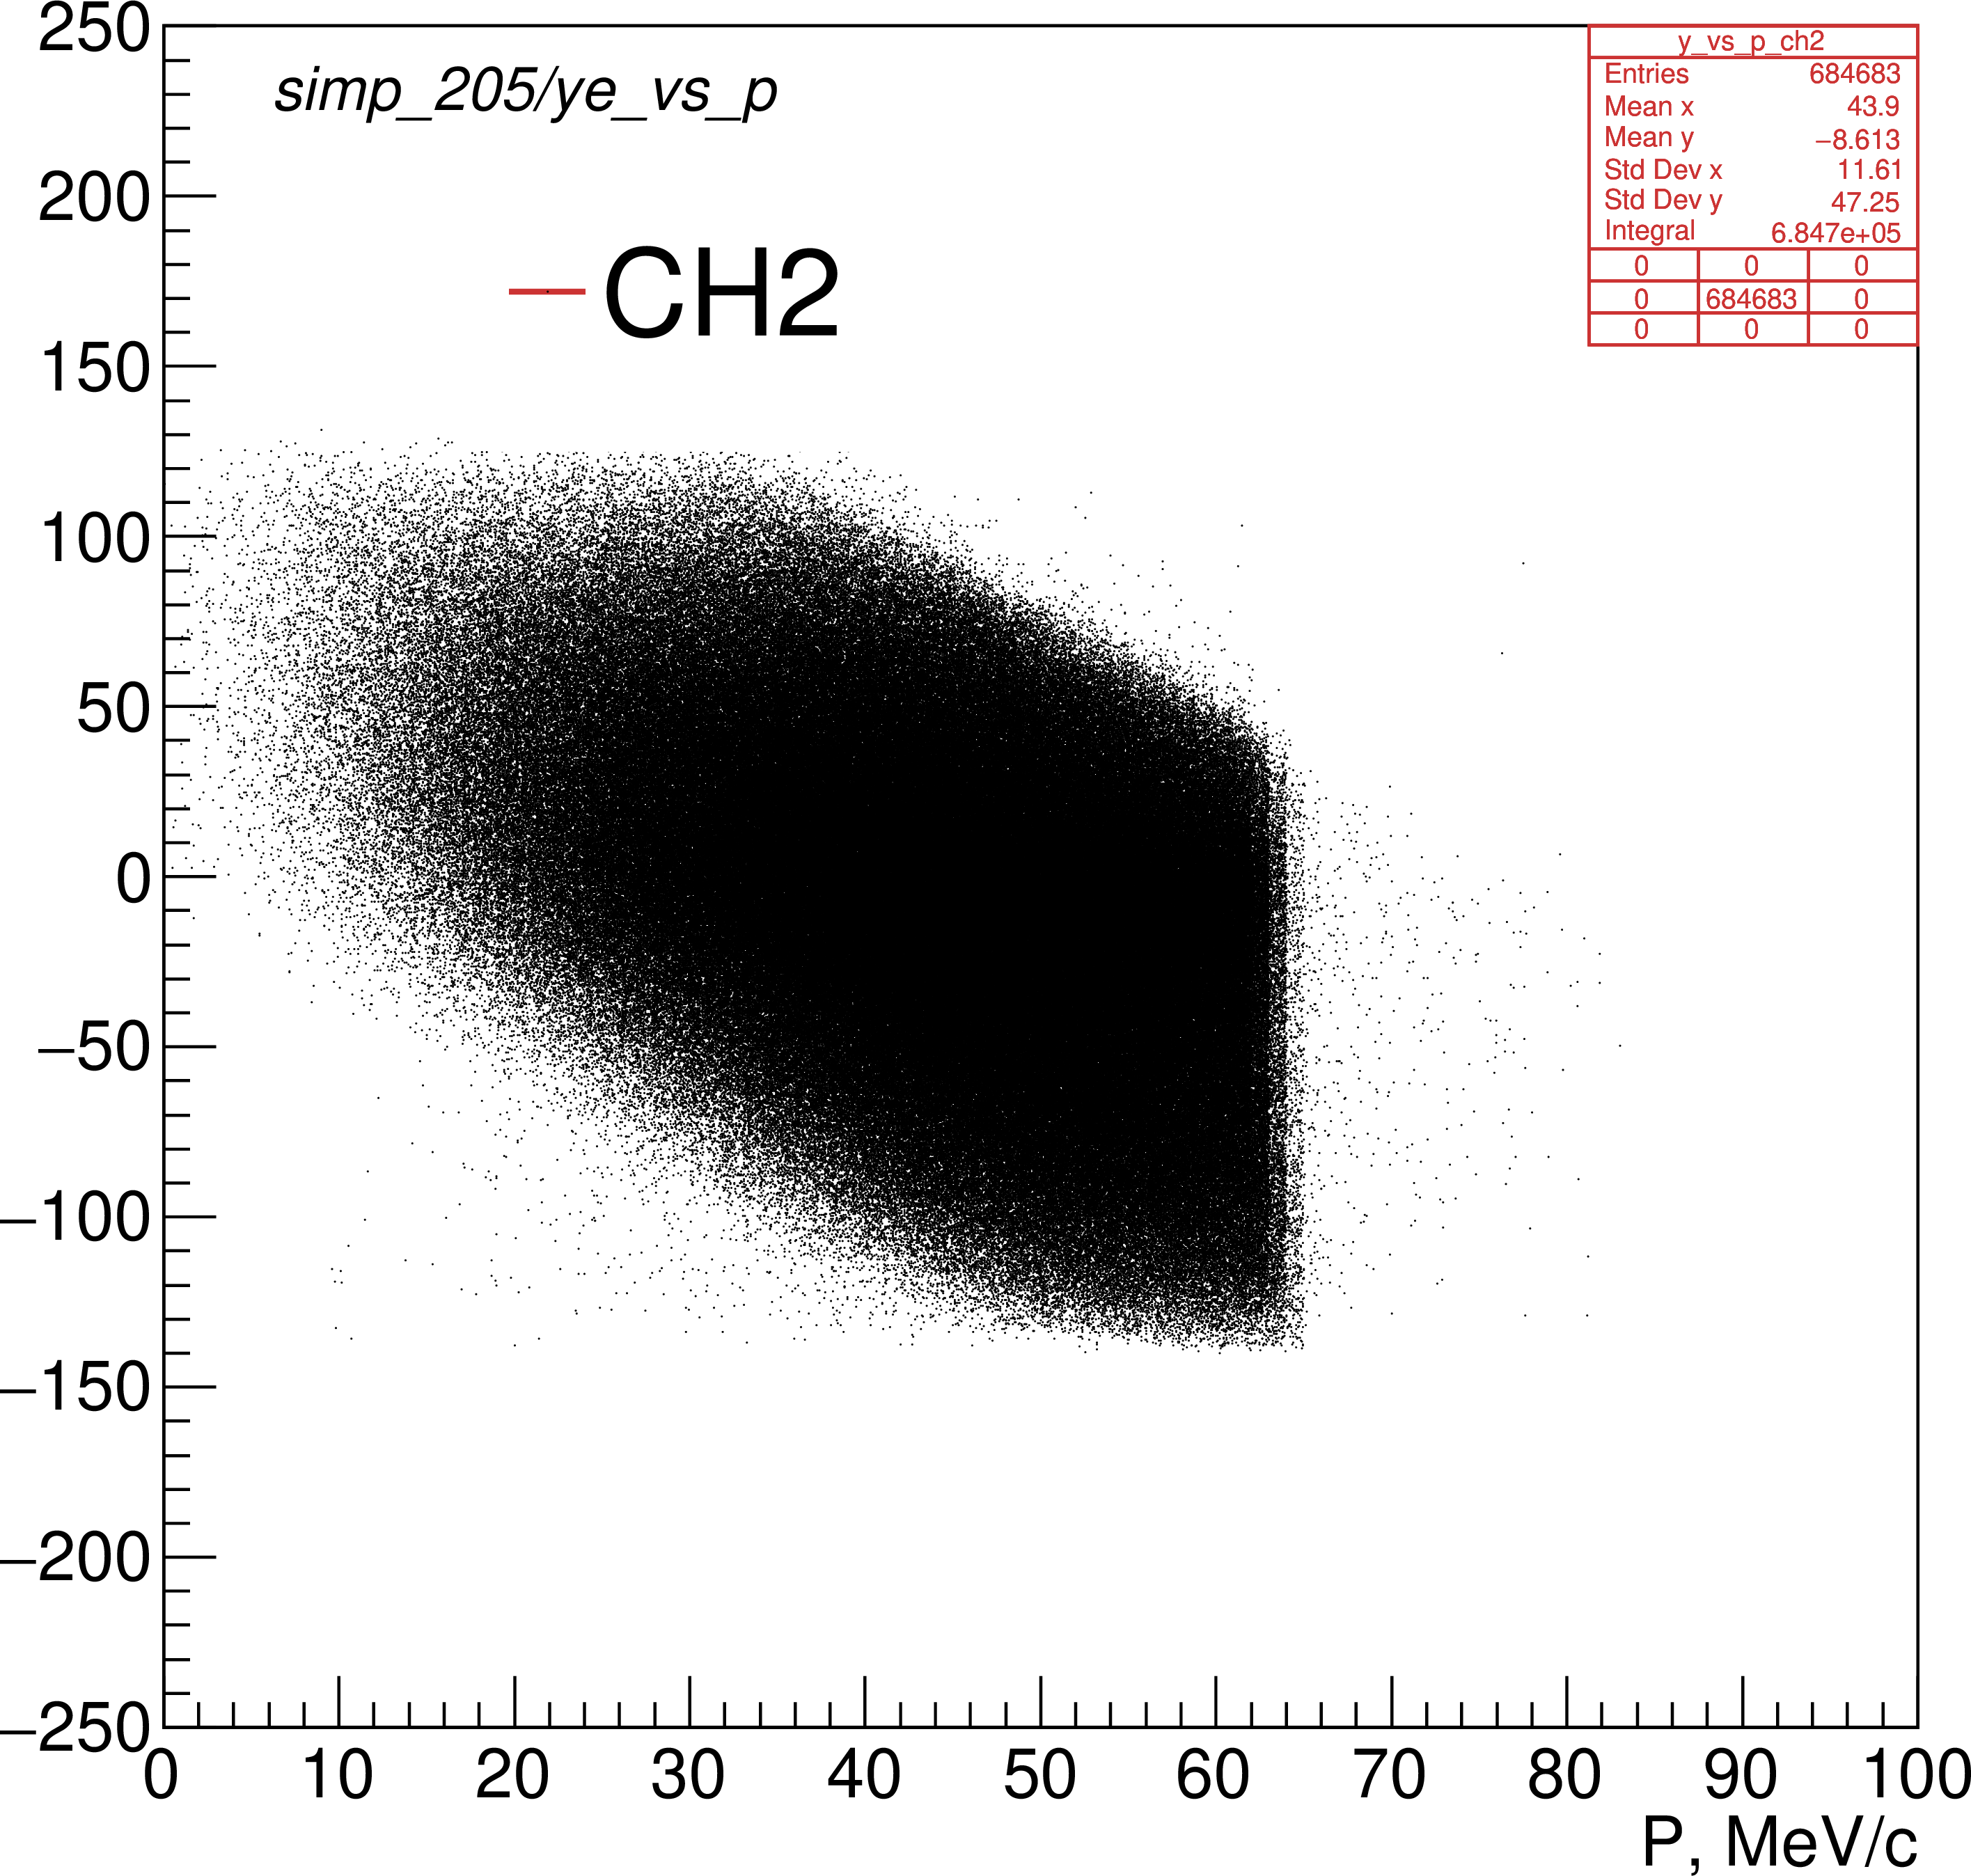
\includegraphics[width=0.5\textwidth]{png/figure_00036}
      %}
    };
    \node[anchor=south west,inner sep=0] at (10.,0.) {
      % \node[shift={(0 cm,0.cm)},inner sep=0,rotate={90}] at (0,0) {}
      % \makebox[\textwidth][c] {
      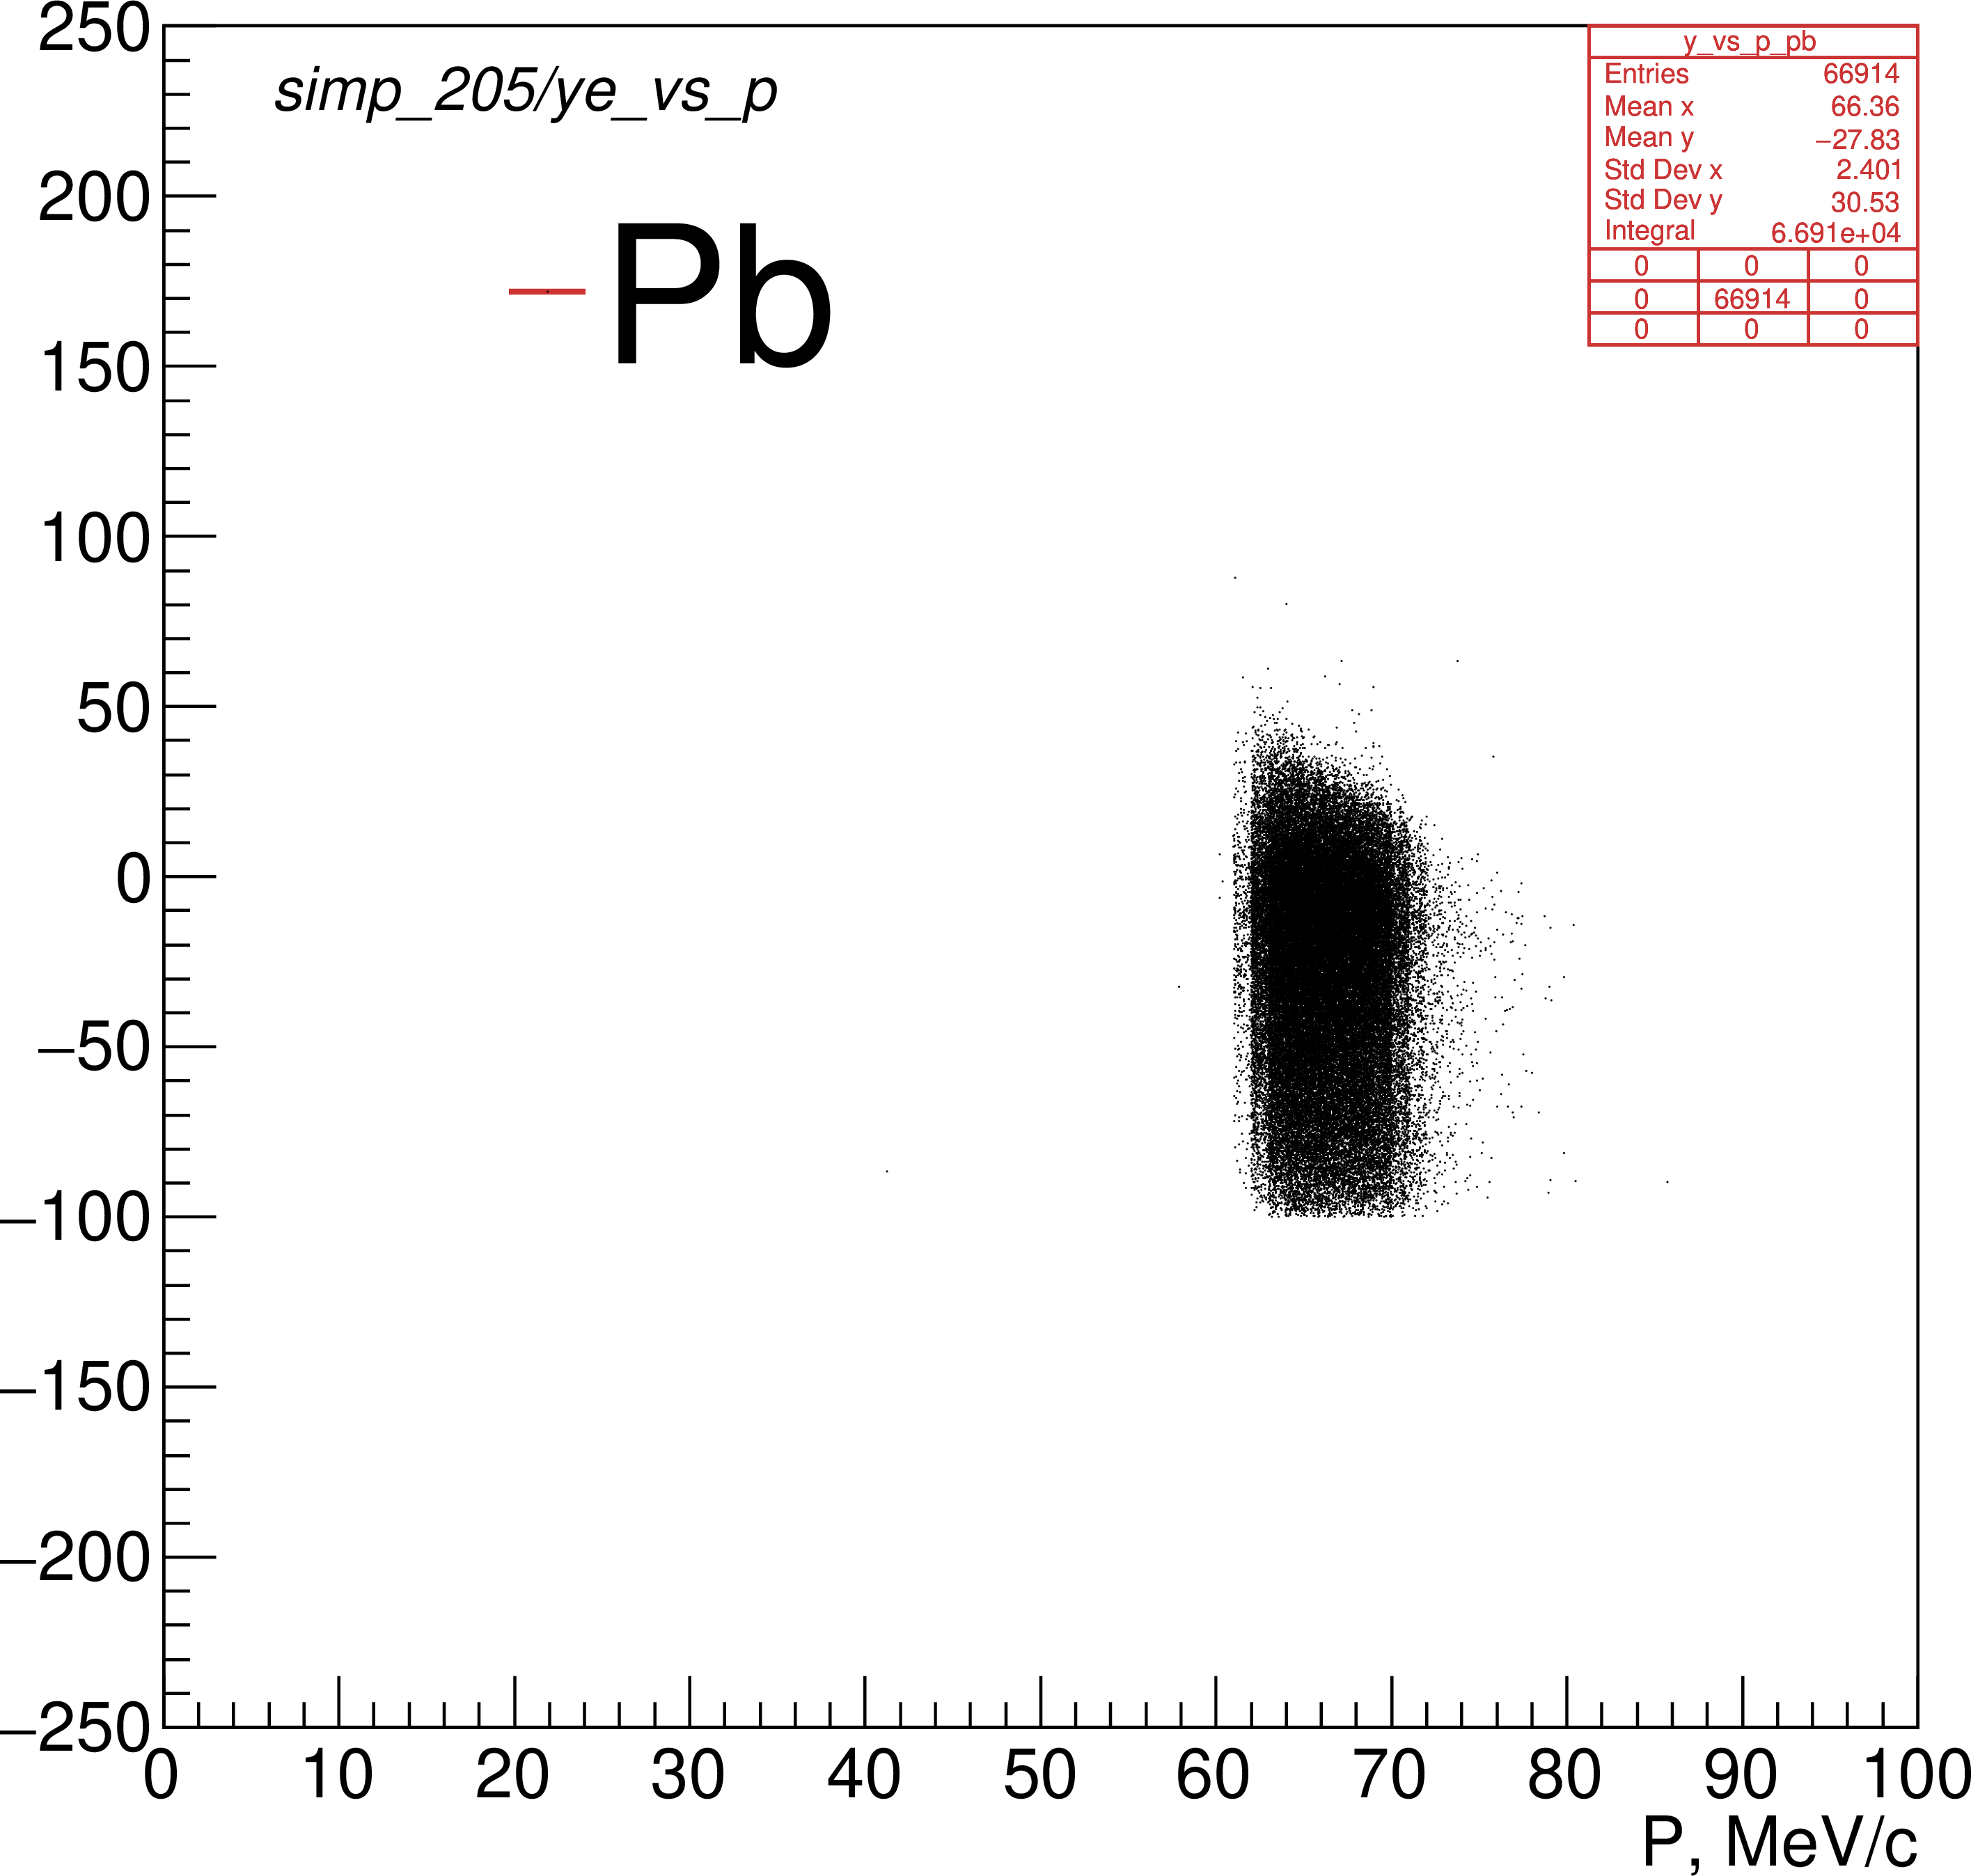
\includegraphics[width=0.5\textwidth]{png/figure_00037}
      %} 
    };
    % \node [text width=8cm, scale=1.0] at (14.5,0.5) {$\mu_B$, expected background mean};
    % \node [text width=8cm, scale=1.0, rotate={90}] at (1.5,7.5) { $S_{D}$, ``discovery'' signal strength  };
  \end{tikzpicture}
  \caption{
    \label{figure:y_vs_p_deg}
    Y(stop):P\@(DS entrance) for negative pions stopped in the $CH_2$ and Pb parts of the simulated degrader
  }
\end{figure}

Y:X distributions of the pion stops in the $CH_2$ disk, Pb foil and the ST are shown in Figure ~\ref{figure:y_vs_x_st}.
They reflect the correlation between the mean Y of the particle trajectory and the particle momentum.

\begin{figure}[H]
  \begin{tikzpicture}
    \node[anchor=south west,inner sep=0] at (0,0.) {
      % \node[shift={(0 cm,0.cm)},inner sep=0,rotate={90}] at (0,0) {}
      %\makebox[\textwidth][c] {
        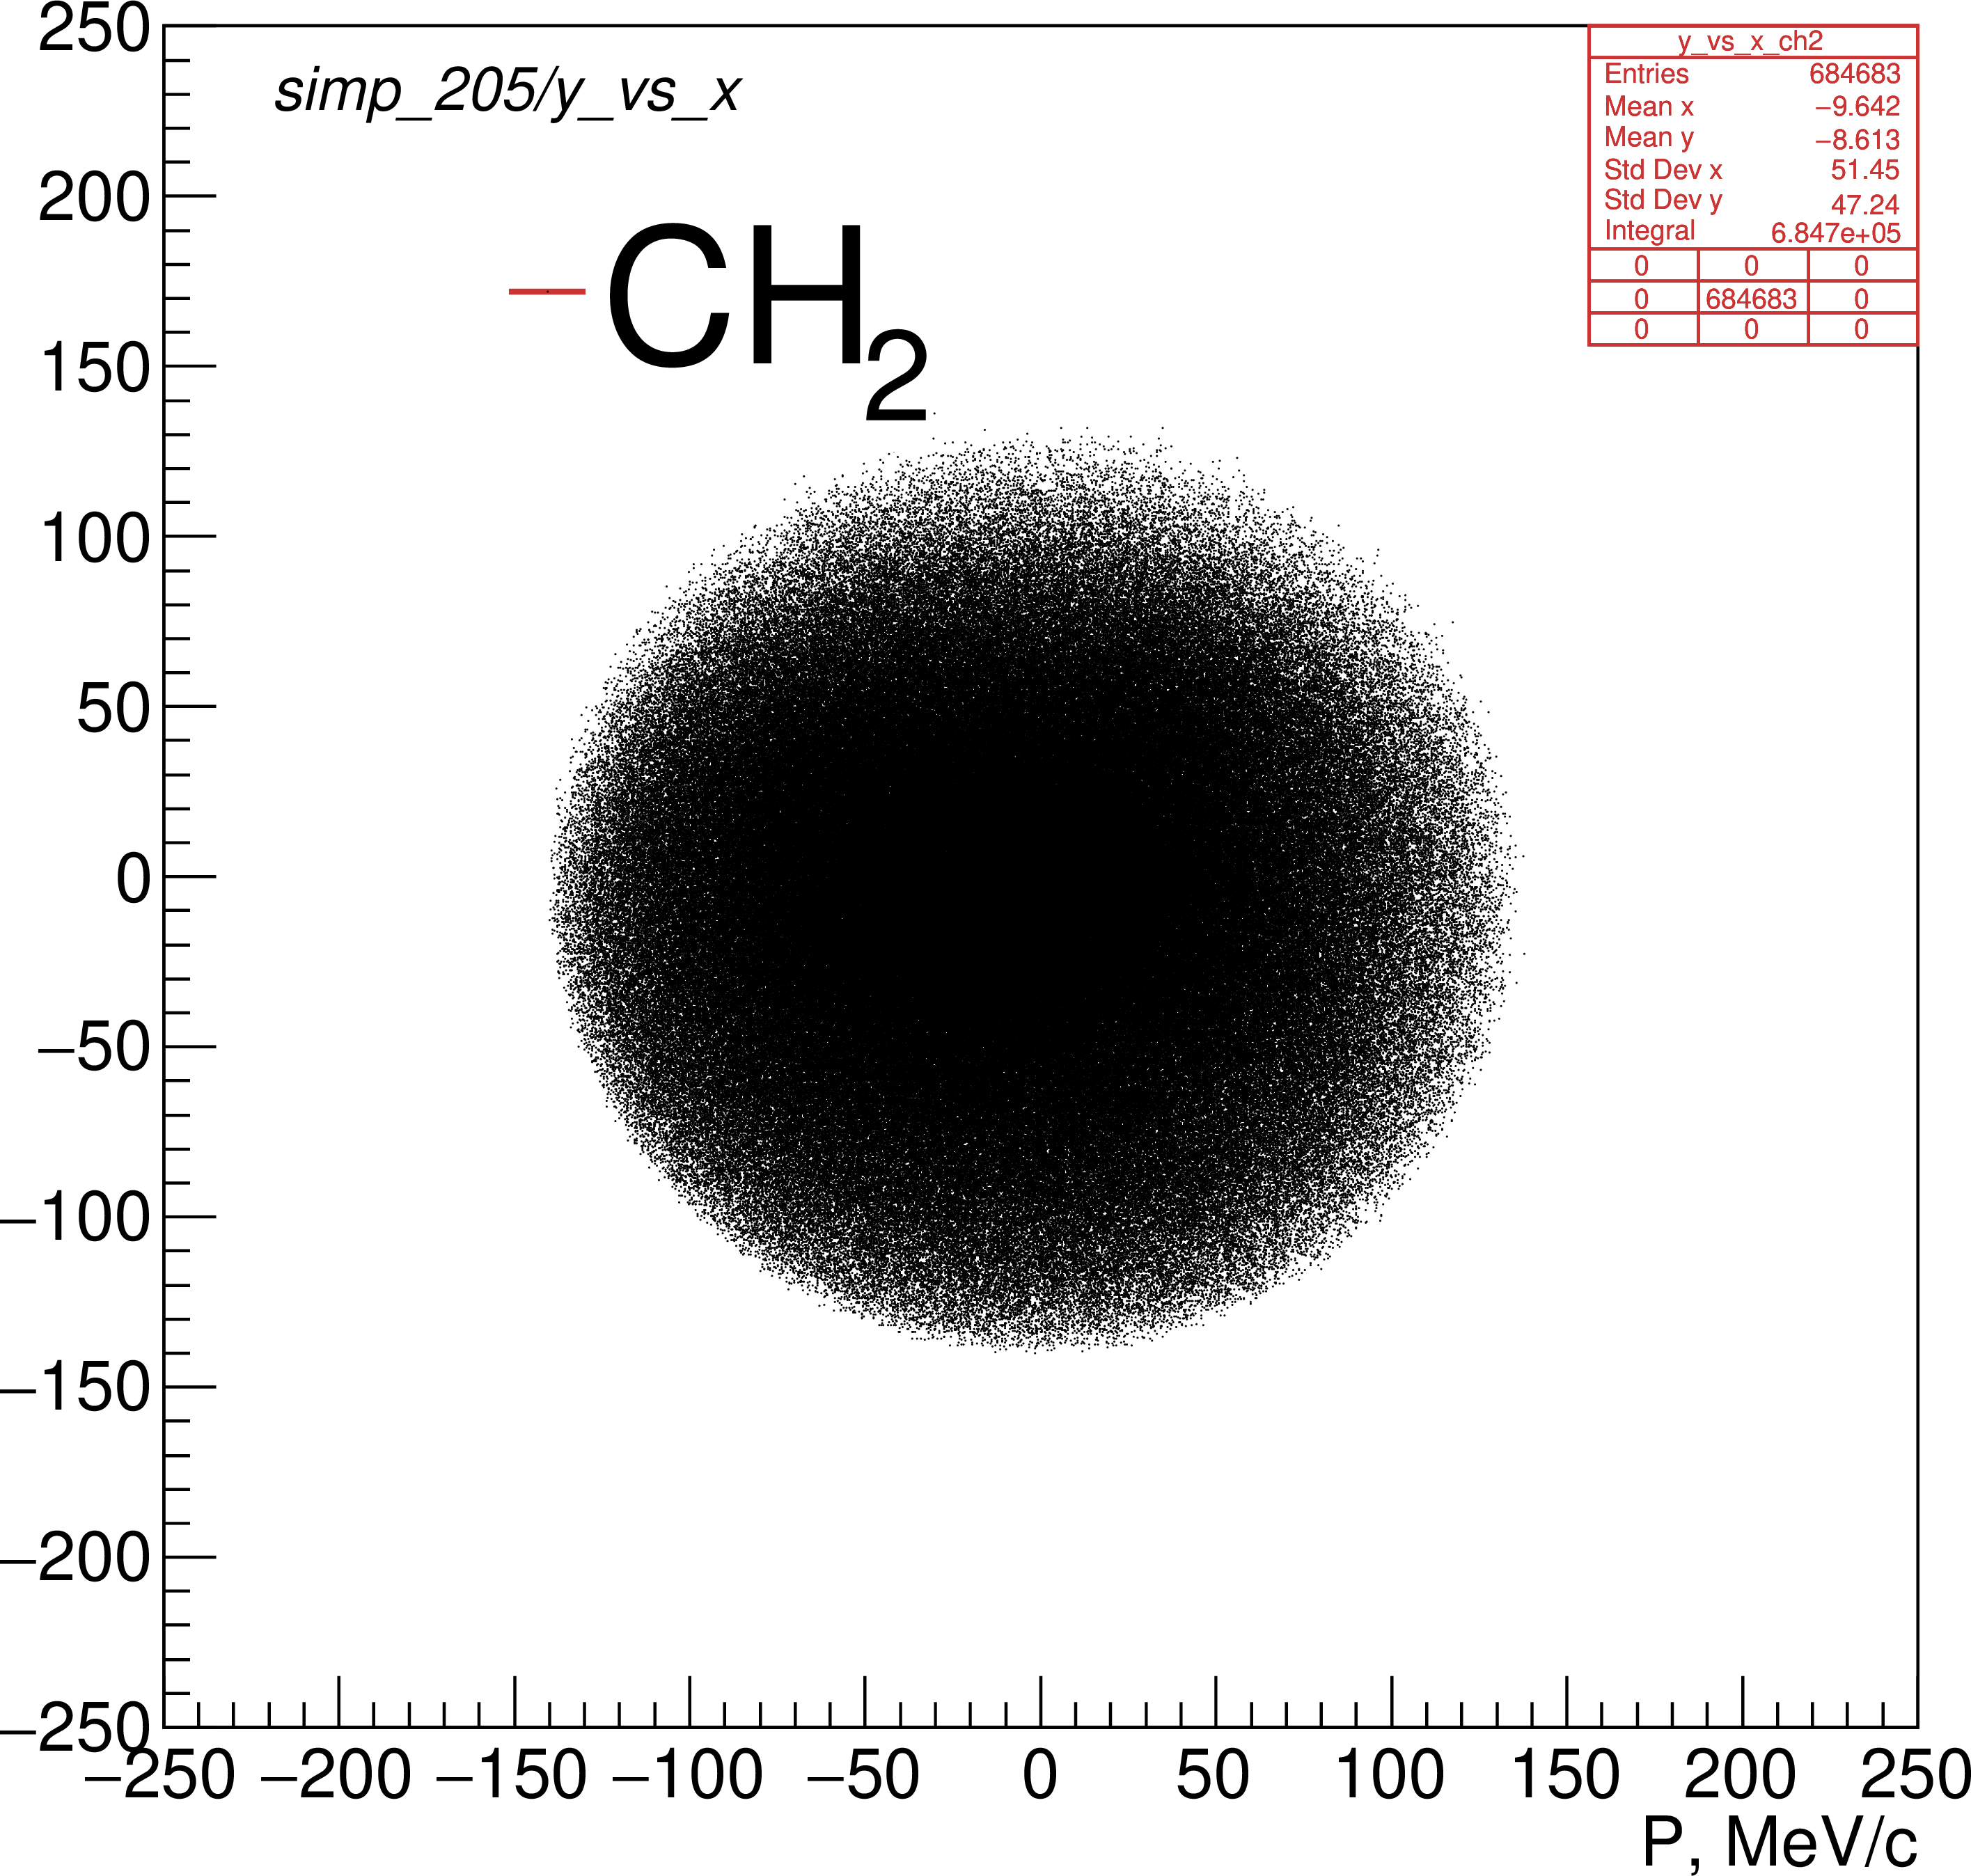
\includegraphics[width=0.5\textwidth]{png/figure_00034}
      %}
    };
    \node[anchor=south west,inner sep=0] at (10.,0.) {
      % \node[shift={(0 cm,0.cm)},inner sep=0,rotate={90}] at (0,0) {}
      %\makebox[\textwidth][c] {
        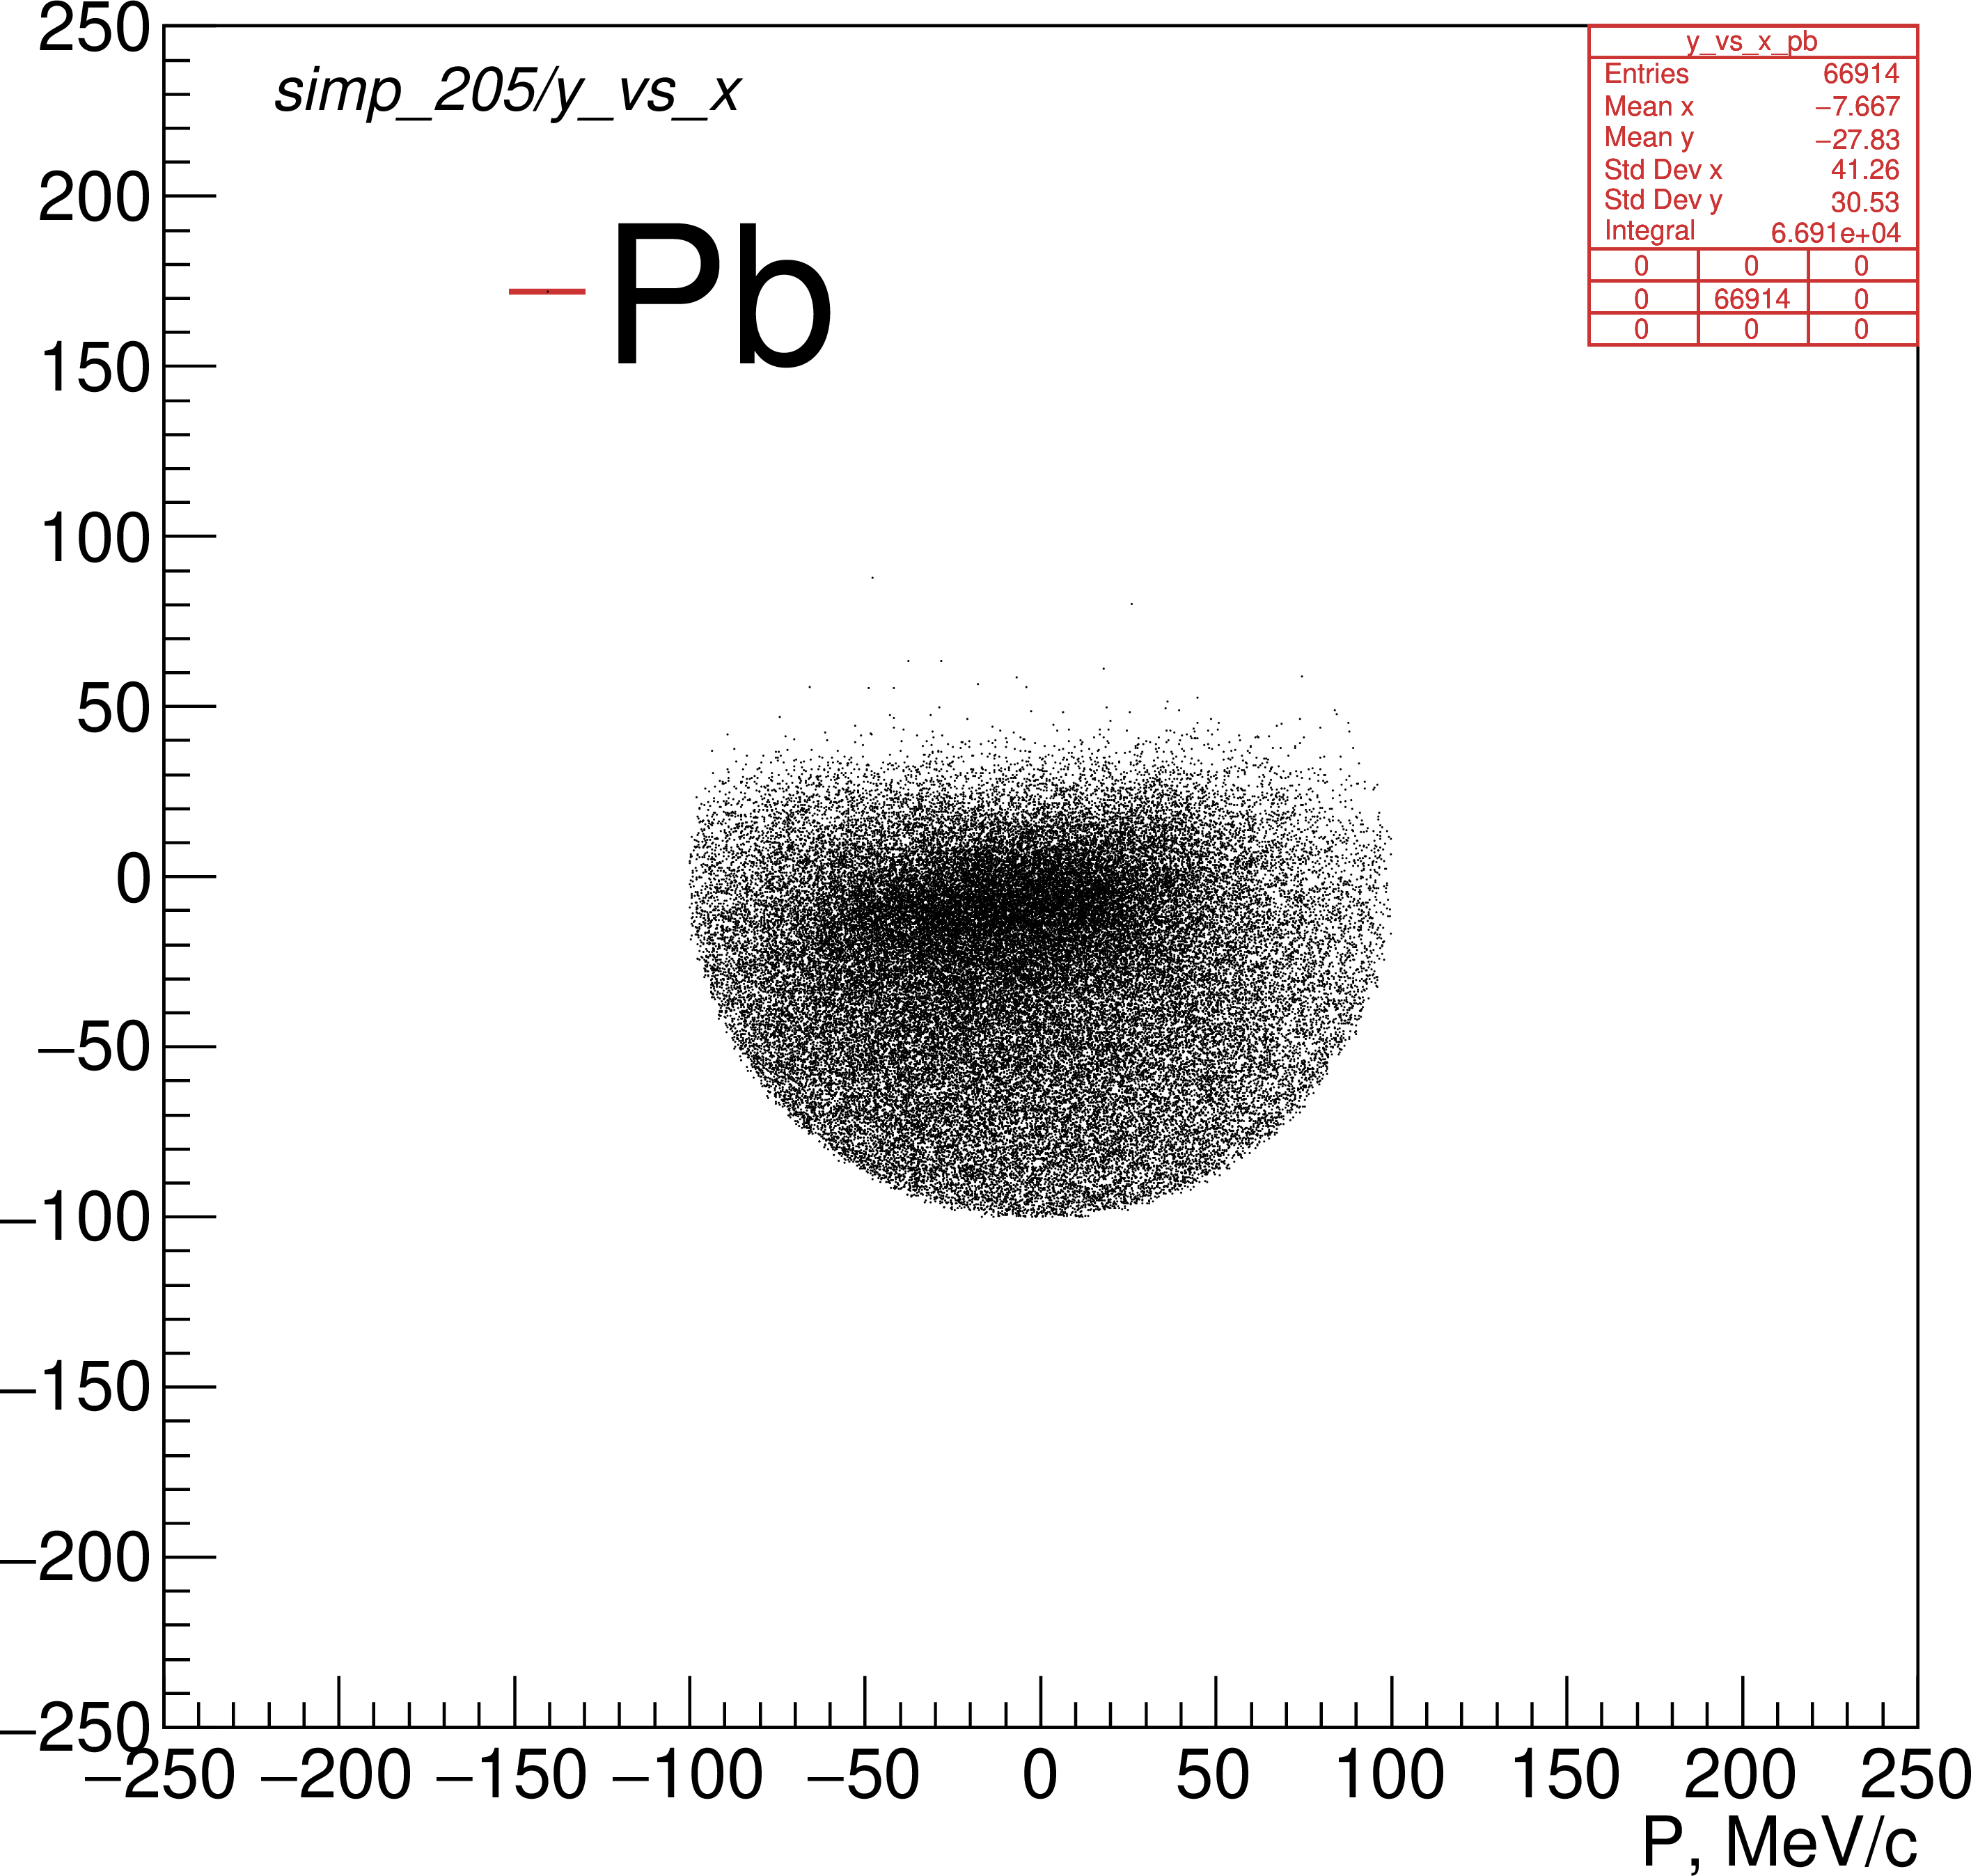
\includegraphics[width=0.5\textwidth]{png/figure_00035}
      %}
    };
    \node[anchor=south west,inner sep=0] at (0,-10.) {
      % \node[shift={(0 cm,0.cm)},inner sep=0,rotate={90}] at (0,0) {}
      % \makebox[\textwidth][c] {
        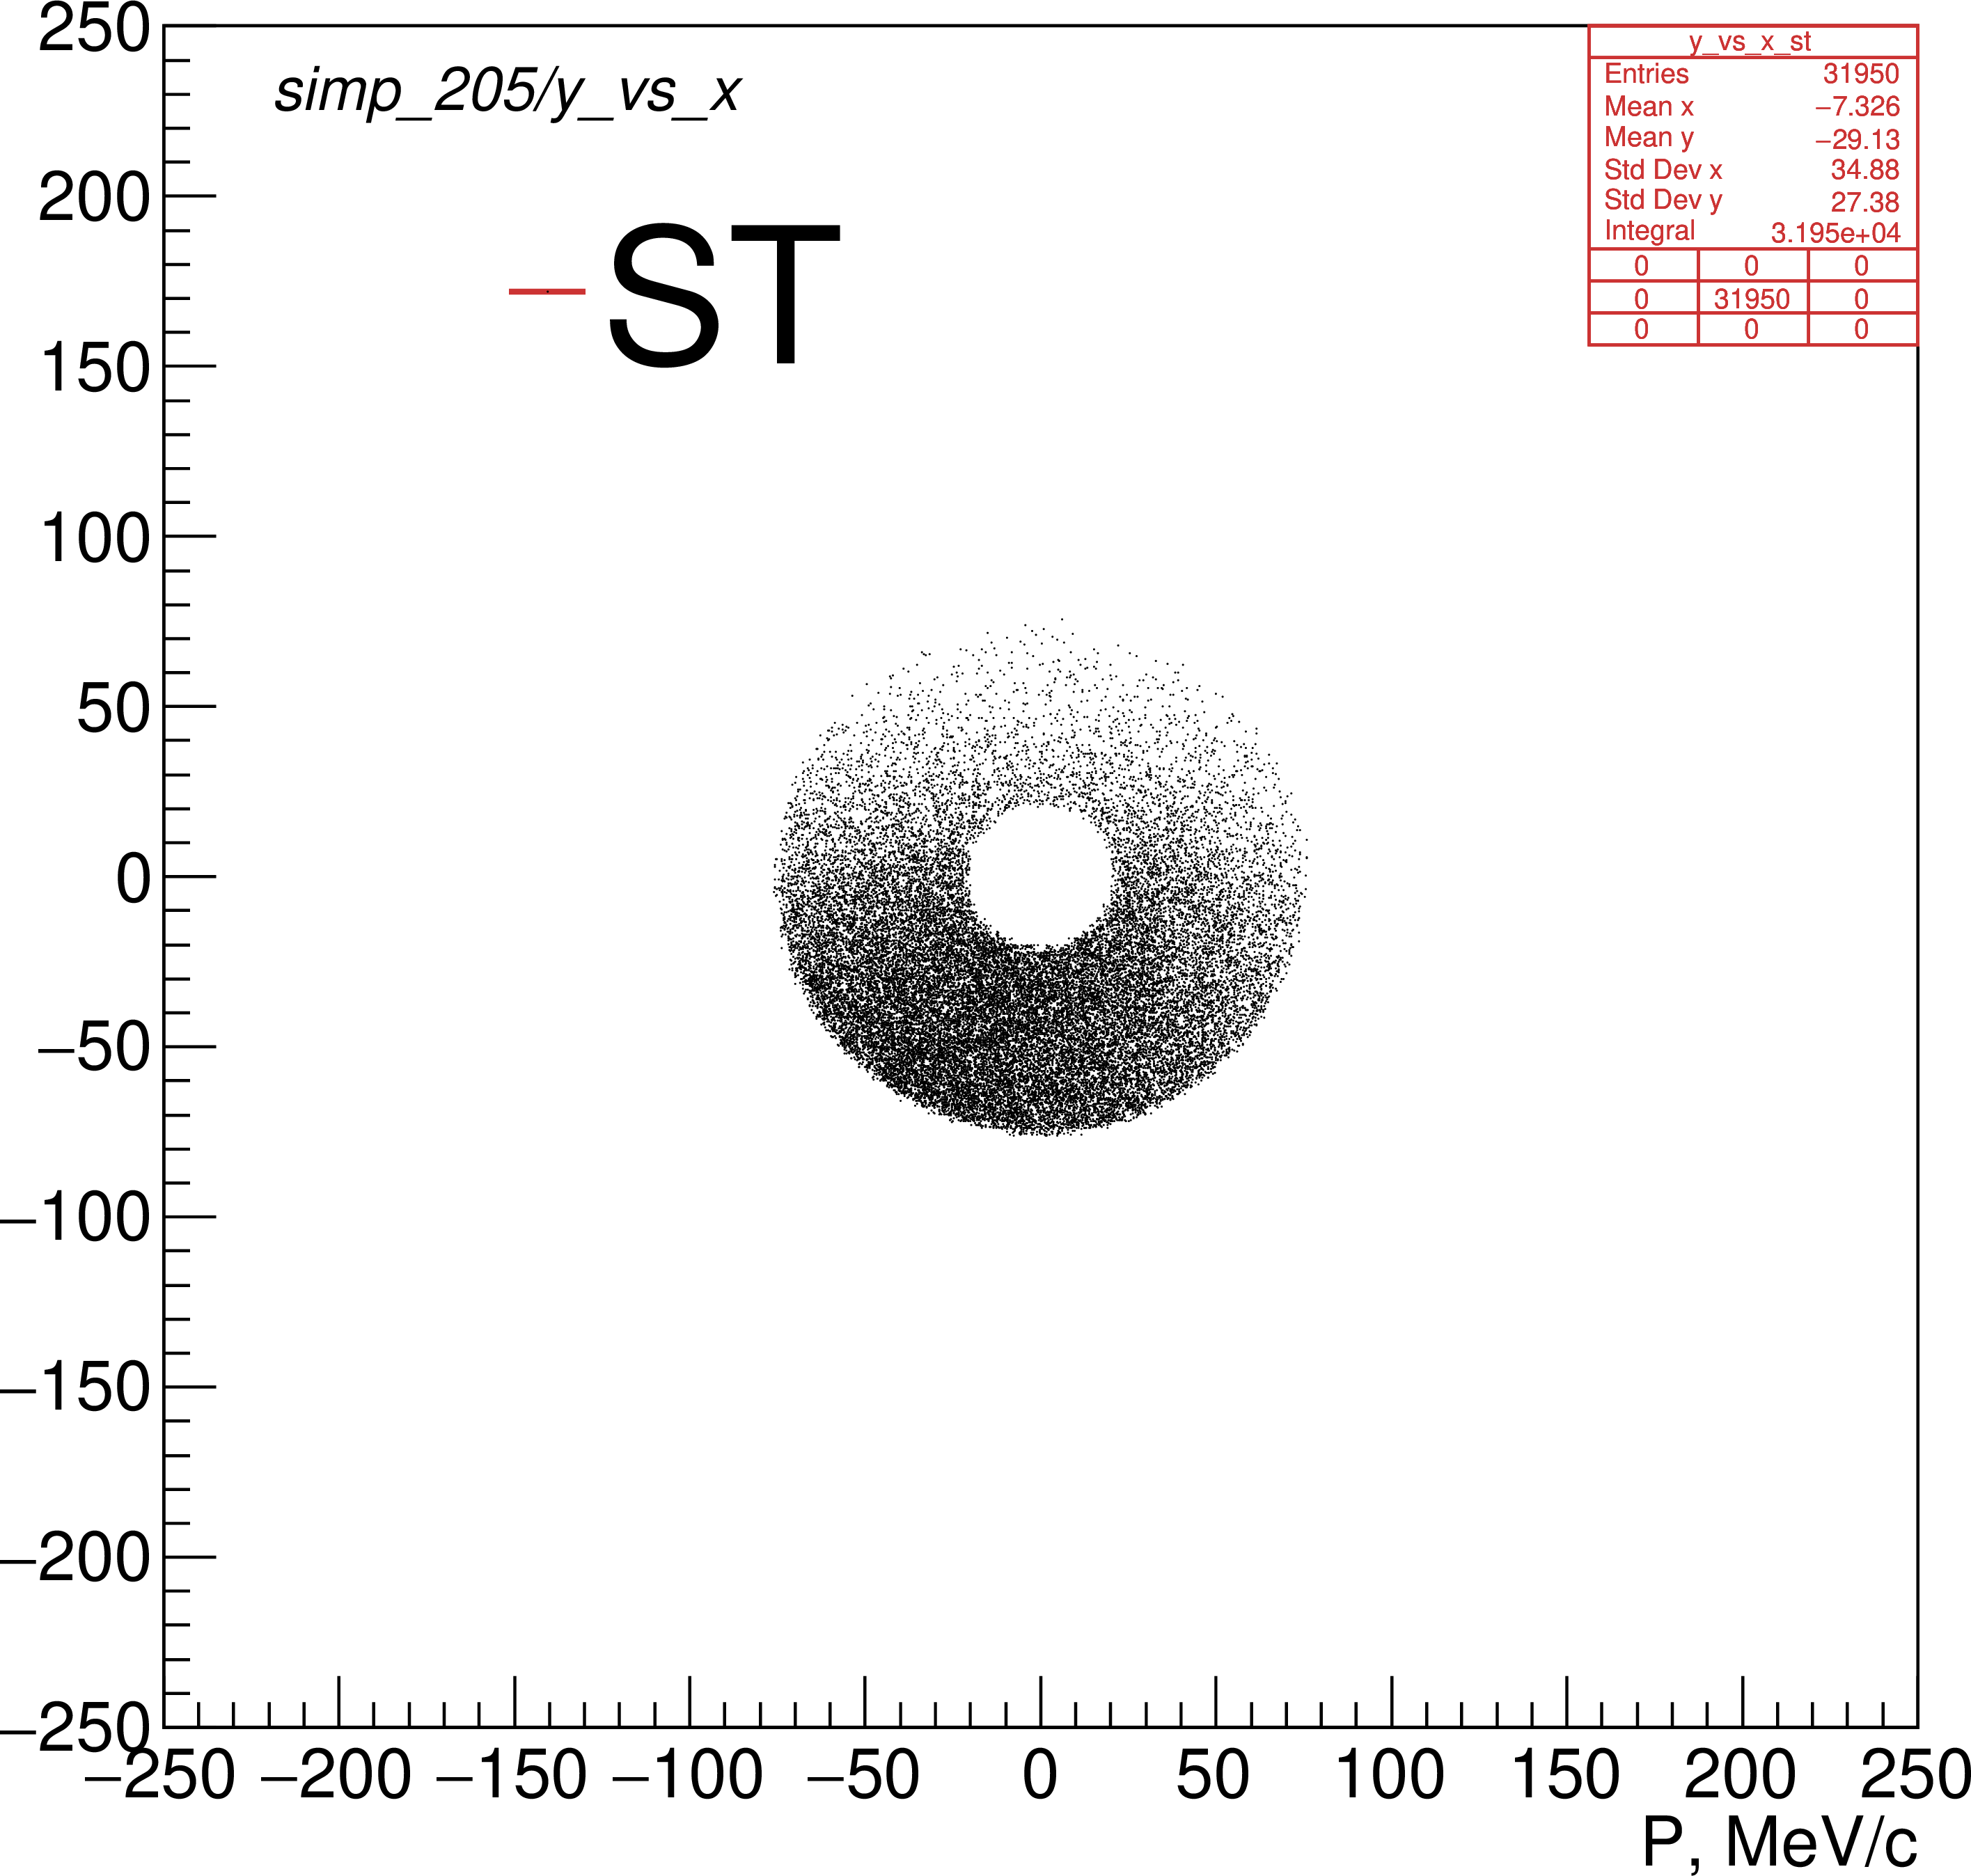
\includegraphics[width=0.5\textwidth]{png/figure_00031}
      % }
    };
    % \node [text width=8cm, scale=1.0] at (14.5,0.5) {$\mu_B$, expected background mean};
    % \node [text width=8cm, scale=1.0, rotate={90}] at (1.5,7.5) { $S_{D}$, ``discovery'' signal strength  };
  \end{tikzpicture}
  \caption{
    \label{figure:y_vs_x_st}
    Y(stop):X(stop) for pions stopped in the CH2, Pb, and ST
  }
\end{figure}


%%% Local Variables:
%%% mode: latex
%%% TeX-master: t
%%% End:

\section{Reconstructed photon spectrum}

For the photon energy of $\sim$ 130 MeV, the present reconstruction code is not expected
to reconstruct $\gamma \to e^+e^-$ events efficiently.

{\red run reconstruction and demonstrate that ? }

However, the intrinsic resolution of the tracker should contribute less than 0.5 MeV to the
reconstructed full width of the $e^+e^-$ conversion peak.

We therefore use the MC truth - the sum of the two MC particle momenta recorded in front
of the tracker - as a proxy to the reconstructed photon momentum
\begin{figure}[H]
  \begin{tikzpicture}
    \node[anchor=south west,inner sep=0] at (0,0.) {
      % \node[shift={(0 cm,0.cm)},inner sep=0,rotate={90}] at (0,0) {}
      \makebox[\textwidth][c] {
        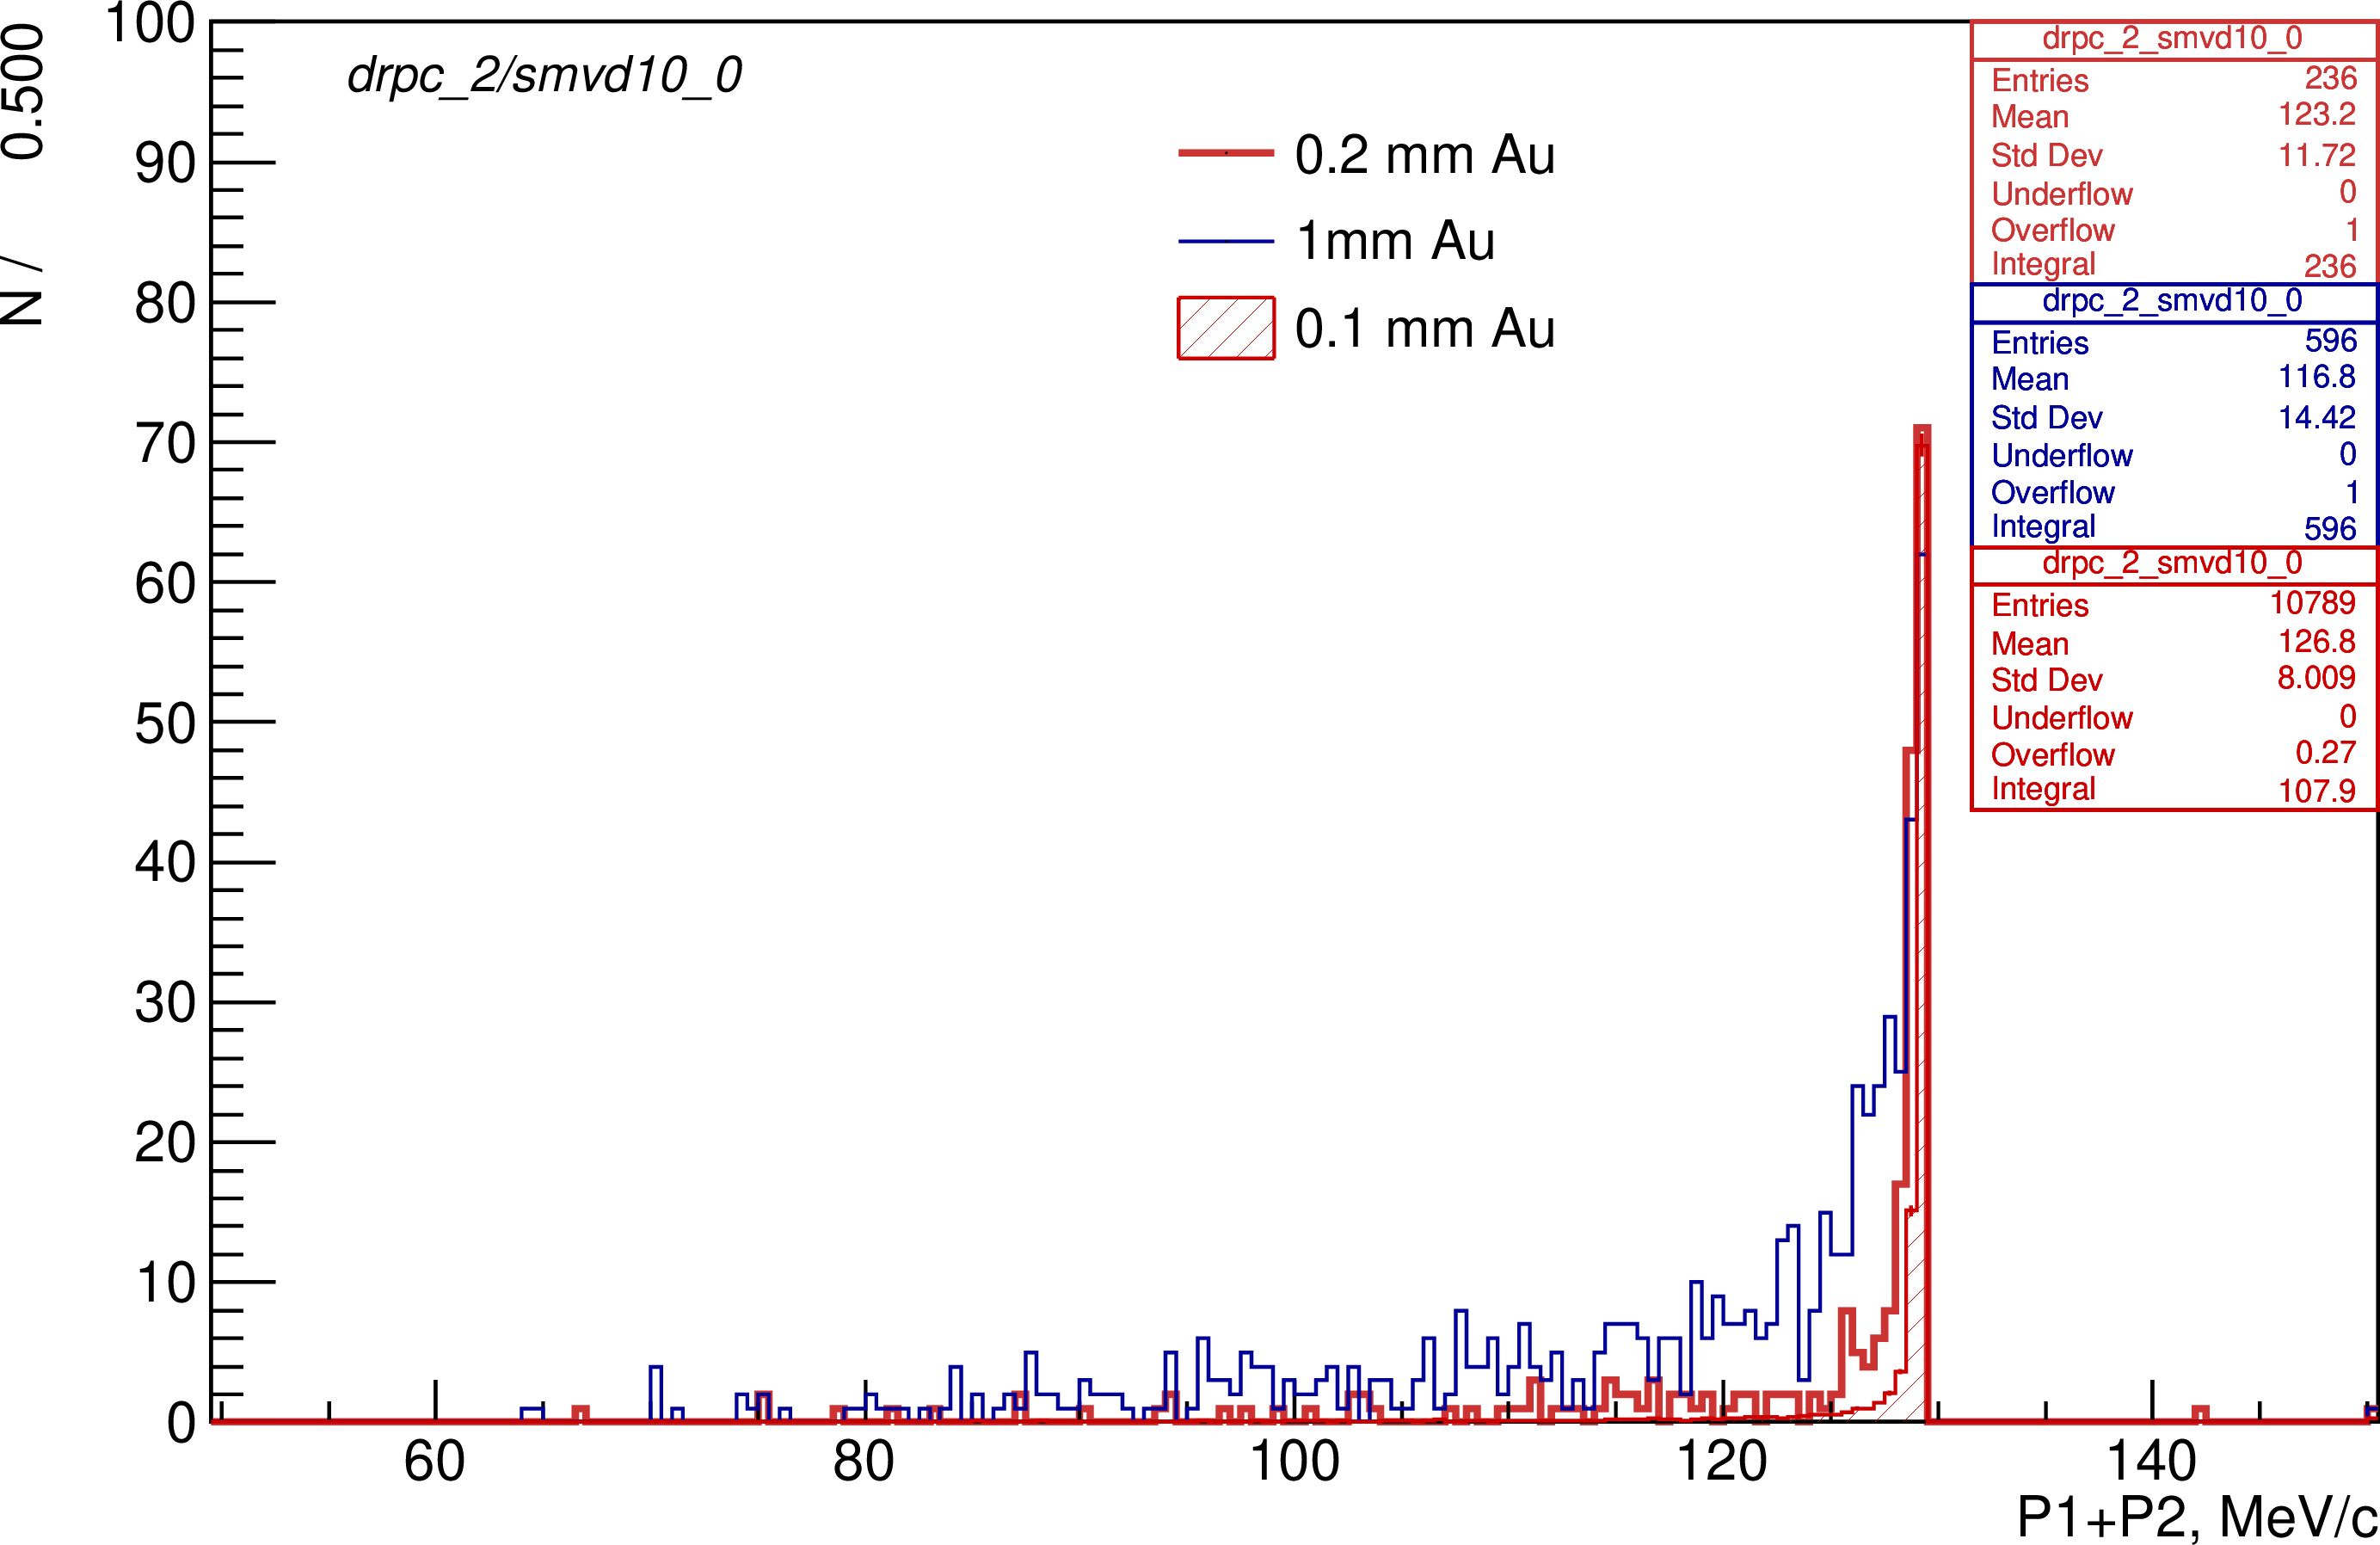
\includegraphics[width=0.9\textwidth]{png/figure_00010}
      }
    };
    % \node [text width=8cm, scale=1.0] at (14.5,0.5) {$\mu_B$, expected background mean};
    % \node [text width=8cm, scale=1.0, rotate={90}] at (1.5,7.5) { $S_{D}$, ``discovery'' signal strength  };
  \end{tikzpicture}
  \caption{
    \label{figure:sum_mom_vd10}
    P1+P2 at VD10
  }
\end{figure}

\begin{figure}[H]
  \begin{tikzpicture}
    \node[anchor=south west,inner sep=0] at (0,0.) {
      % \node[shift={(0 cm,0.cm)},inner sep=0,rotate={90}] at (0,0) {}
      \makebox[\textwidth][c] {
        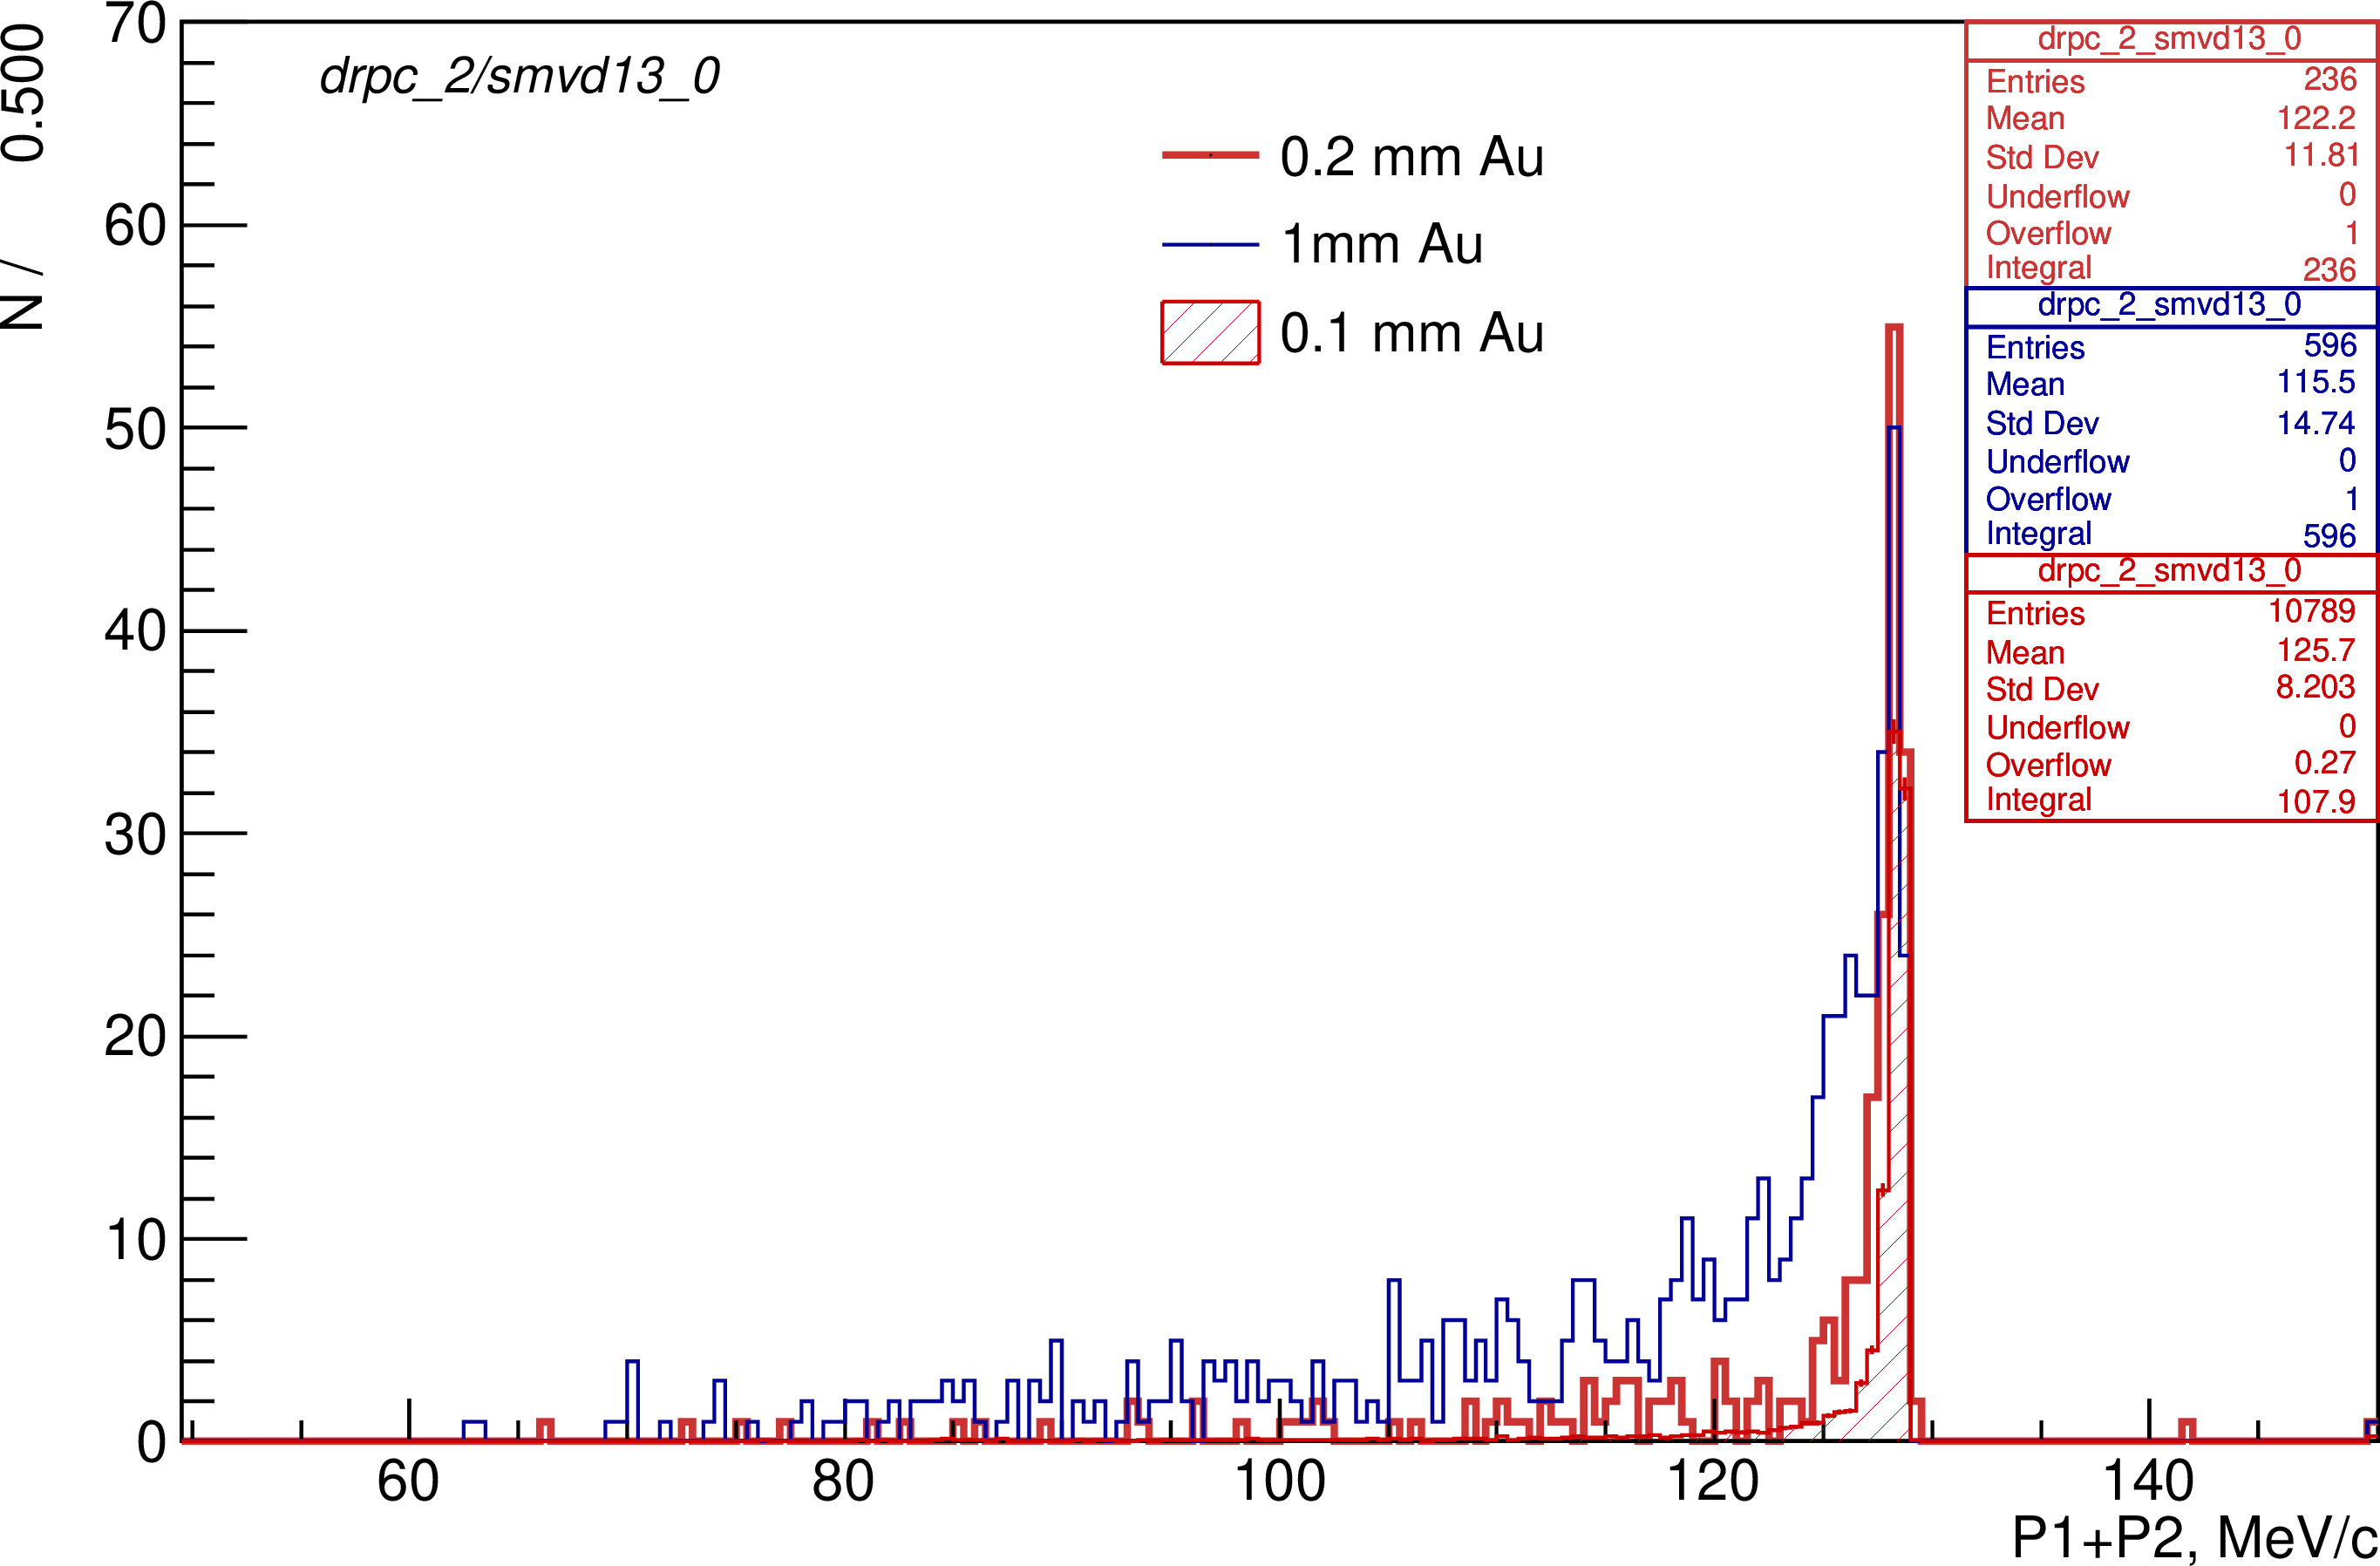
\includegraphics[width=0.9\textwidth]{png/figure_00013}
      }
    };
    % \node [text width=8cm, scale=1.0] at (14.5,0.5) {$\mu_B$, expected background mean};
    % \node [text width=8cm, scale=1.0, rotate={90}] at (1.5,7.5) { $S_{D}$, ``discovery'' signal strength  };
  \end{tikzpicture}
  \caption{
    \label{figure:sum_mom_vd13}
    P1+P2 at VD09, VD10, VD13
  }
\end{figure}

The converter thickness is chosen based on the distributions shown in Figure~\ref{figure:sum_mom_vd13}.
Plotted: $P_{tot} = P_1 + P_2$ at VD13, virtual detector in front of the tracker fro events with
two particles, an electron and a positron with P > 30 MeV/c and producing 20 or more straw hits in the tracker each.
Such particles provide a good proxy to the reconstructable tracks.

The event yield increases with the converter thickness. However of interest for the scale calibration only
are the events close to the kinematic edge.
The highest yield of events with P > 128 Mev/c corresponds to the 100 um gold foil, and that determines
the choice of 100 um thick converter.

\begin{figure}[H]
  \begin{tikzpicture}
    \node[anchor=south west,inner sep=0] at (0,0.) {
      % \node[shift={(0 cm,0.cm)},inner sep=0,rotate={90}] at (0,0) {}
      \makebox[\textwidth][c] {
        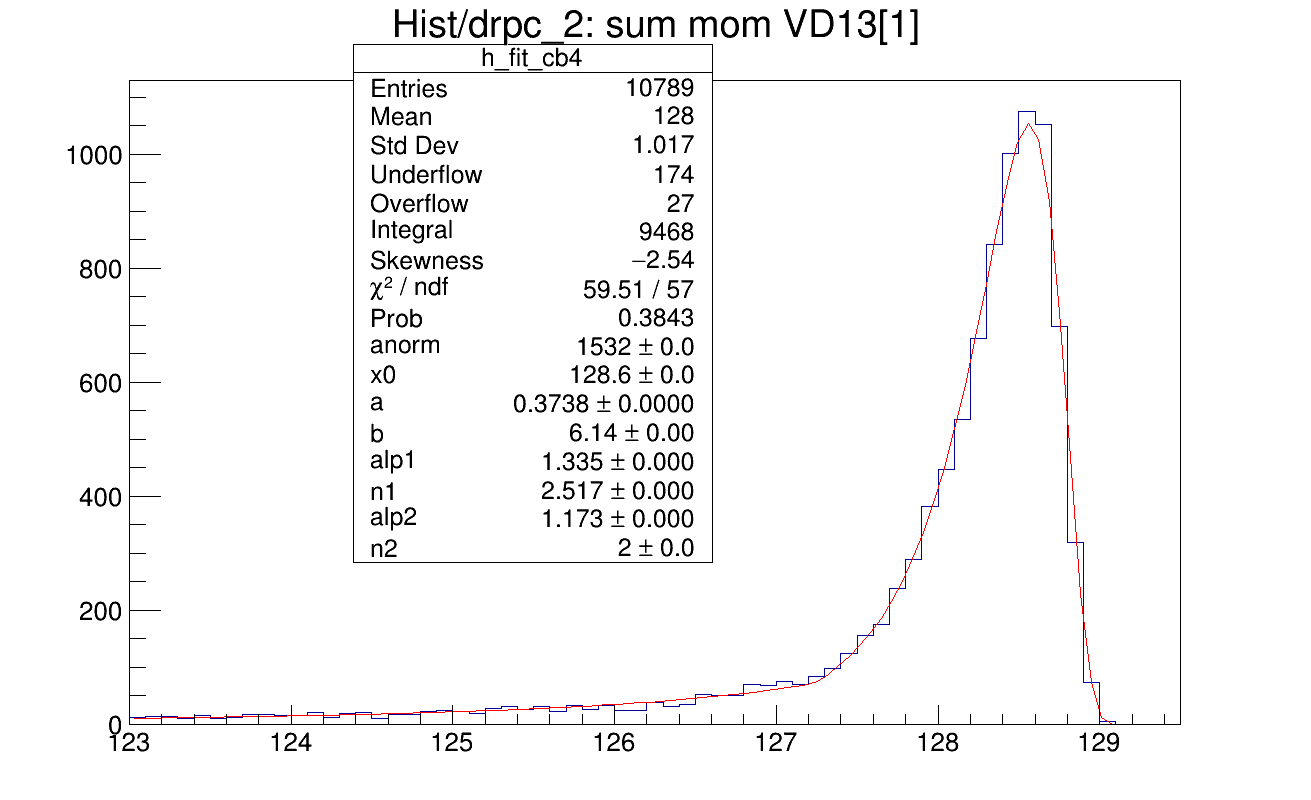
\includegraphics[width=0.9\textwidth]{png/pipenu_bpip4b0_murat_track_ana_trk_0_p_fit}
      }
    };
    % \node [text width=8cm, scale=1.0] at (14.5,0.5) {$\mu_B$, expected background mean};
    % \node [text width=8cm, scale=1.0, rotate={90}] at (1.5,7.5) { $S_{D}$, ``discovery'' signal strength  };
  \end{tikzpicture}
  \caption{
    \label{figure:sum_mom_vd09_10_13}
    P1+P2 at VD09, VD10, VD13
  }
\end{figure}

Figure ~\ref{figure:sum_mom_vd09_10_13} shows the $P_{tot}$ distribution for 100 um converter
with the binning of 100 keV/c. The most probable energy loss is about 800/c keV, 
and the resolution function has the FWHM of about 700 keV/c.
These numbers are not very different from the same numbers for conversion electrons.

Assuming that, similar to the CE case, the width of the distribution is dominated by the energy losses,
the reconstructed $\gamma \to e^+e^-$ peak will have the FWHM $\simeq 1$ MeV/c and the offset
of about 1 MeV from its nominal position.

{\red need fit uncertainties to estimate the uncertainty on the edge position }

%%% Local Variables:
%%% mode: latex
%%% TeX-master: t
%%% End:


%%%%%%%%%%%%%%%%%%%%%%%%%%%%%%%%%%%%%%%%%%%%%%%%%%%%%%%%%%%%%%%%%%%%%%%%%%%%%%
\section{Electric current}
When inserted into the beam, the degrader stops the beam particles, mostly electrons.
Therefore, to avoid the charge accumulation, the degrader needs to be grounded.
An estimate of the electric current can be obtained as follows:
\begin{itemize}
\item
  assume that degrader stops all beam flash particles
\item
  from SU2020: the rate of the beam flash particles, assume all are electrons, is $\sim ~ 10^2$ of that of muons
\item
  muons : $1.6 \cdot 10^{-3} \times 3.9 \cdot 10^7$ , say, $7 \cdot 10^4$, which gives $\sim ~ 7 \cdot 10^7$ electrons per 1.7 ms
\item
  the corresponding electric current is $I ~=~ 7 \cdot 10^{-7} \times 1.6 \cdot 10^{-19} / {1.7 \cdot 10^{-6}} \sim 7 \cdot 10^{-6}$ A,
  or $\sim$ 10 microamperes
\end{itemize}




%%%%%%%%%%%%%%%%%%%%%%%%%%%%%%%%%%%%%%%%%%%%%%%%%%%%%%%%%%%%%%%%%%%%%%%%%%%%%%
\section{Estimate of the time needed for momentum calibration}
Calibration with RPC on hydrogen allows to determine the momentum scale of the experiment.

In this section we assume that the experimental background doesn't affect
the determination accuracy of the momentum edge of RPC photon peak
and estimate the time needed for the calibration.

\begin{itemize}
\item 
From $ 2.5 \times 10^8 $ protons on target, 67.42 negative pions stop on the $\rm{CH_2}$ part of the degrader at T>200ns.
\item 
  A negative pion stopped in $\rm{CH_2}$ has a probability of about $ 5 \times 10^{-3} $ of producing a 129.4 MeV RPC photon from capture on hydrogen (Section 3).
\item 
The optimal geometry from Section 4 places a gold converter at radius R=25.0cm with thickness 0.1mm. Of $10^7$ RPC photons generated with angle 0<$\cos \theta$<0.2, 10789 produce $e^+ e^-$ pairs that can likely be reconstructed in the tracker (Section 5). Events counted as likely reconstructable have $e^+$ and $e^-$ each with at least 20 straw hits and momentum P > 30MeV/c. Scaling to the full range of photon angles reduces the yield by a factor of 0.2/2, to around $10^{-4}$  per RPC photon. 
\end{itemize}
The product of these first three factors is a calibration event rate on the order of $10^{-13} $ per POT.

\begin{itemize}
\item 
  required accuracy of the momentum scale calibration $@$100 MeV/c: $\sigma_P/P$ < 100 keV/c
\item
Estimates in the remaining items assume that reconstructed tracks from 1000 $ \gamma \to e^+ e^- $ events would be sufficient to reconstruct the high-energy edge of the 129.4 MeV RPC photon momentum distribution. Examples are the fitted peaks in Sections 6-7, which both have about 1000 events in the tracker using the default reconstruction.  
\item
For a yield of $10^{-13}$ events/POT, collecting 1000 events requires $10^{16}$ protons on target.
  In one-batch mode, an average expected pulse intensity is $1.6 \times 10^7$, with one pulse every 1695ns for about 0.4s of each 1.4s Main Injector cycle. The resulting rate is $2.7 \times 10^{12}$ protons/sec, which would provide 1000 calibration events in less than an hour.
\item
  Assuming that calibration data is taken at 10\% of nominal beam intensity with a data collection efficiency of 50\%, the time needed increases by a factor of 20. A further reconstruction efficiency factor of 50\% takes into account events not reconstructed in the tracker, an estimate for the case after improving reconstruction efficiency. Overall, collecting 1000 reconstructable $ \gamma \to e^+ e^- $ events would require on the order of $10^5$ seconds, or about one day of running.
\item
  running at 10\% of the nominal beam intensity in one-batch mode and with the digitization starting
  at 200 ns corresponds to the total number of background hits per microbunch of about 200,
  so the pileup at T>300 ns should not be a problem.
\end{itemize}


%%% Local Variables:
%%% mode: latex
%%% TeX-master: t
%%% End:


%%%%%%%%%%%%%%%%%%%%%%%%%%%%%%%%%%%%%%%%%%%%%%%%%%%%%%%%%%%%%%%%%%%%%%%%%%%%%% 
\section {Summary}

to be written
%%%%%%%%%%%%%%%%%%%%%%%%%%%%%%%%%%%%%%%%%%%%%%%%%%%%%%%%%%%%%%%%%%%%%%%%%%%%%%
%
%%%%%%%%%%%%%%%%%%%%%%%%%%%%%%%%%%%%%%%%%%%%%%%%%%%%%%%%%%%%%%%%%%%%%%%%%%%%%%
\newpage
\bibliographystyle{unsrtnat}
\bibliography{clfv,mu2e_internal_notes,mu2e_piplusenu_notes,radiative_pion_capture}

% \include{appendix_a}
\appendix

%%%%%%%%%%%%%%%%%%%%%%%%%%%%%%%%%%%%%%%%%%%%%%%%%%%%%%%%%%%%%%%%%%%%%%%%%%%%%%
\section {Datasets}
\label{appendix_b}

\begin{itemize}
\item 
  Definition of the datasets used for this study and the book-keeping information
  can be found at \\
  \href{https://github.com/sridhar130/pipenu/blob/main/doc/datasets.org}
  {\blue https://github.com/sridhar130/pipenu/blob/main/doc/datasets.org}.
\item
  the datasets and stntuples are available from {\bf mu2egpvm*:/exp/mu2e/data/projects/pipenu}
\item
  location of the stntuple catalogs : \\
  \href{https://mu2e.fnal.gov/public/hep/computing/Stntuple/cafdfc/pipenu/index.shtml}
  {\blue https://mu2e.fnal.gov/public/hep/computing/Stntuple/cafdfc/pipenu/index.shtml}
\end{itemize}

%%% Local Variables:
%%% mode: latex
%%% TeX-master: t
%%% End:


\end{document}
